\documentclass[12pt,a4paper,notitlepage]{report}
\usepackage[utf8]{inputenc}
\usepackage{amsmath}
\usepackage{amsfonts}
\usepackage{amssymb}
\usepackage{graphicx}
\usepackage{cite}
\usepackage{textcomp}
\usepackage{url}

\usepackage{caption}

\usepackage[toc,page]{appendix}
\usepackage{hyperref}

\usepackage[left=2cm,right=2cm,top=2cm,bottom=2cm]{geometry}
\title{}
\author{}
\date{}
\begin{document}

\chapter*{Literature Review}

\section*{Tracking user movement}

An obvious way to track user position is to perform double integration on the obtained acceleration to get distance travelled. However this results in introduction of error due to being only an approximation of the underlying signal. Furthermore, integration of the noise component leads to the standard deviation of the error in position increasing with integration time~\cite[p.73]{integrationError}. Thong, Y. K., et al.~\cite{integrationErrorPractical} analysed the practical effect that double integration of accelerometer noise has on this error by carrying out experiments using two commercial accelerometers, and found that this error very quickly accumulates with time~\cite[p.1168]{integrationErrorPractical}. Hence this approach is unsuitable for a navigation system which continuously and precisely requires the user’s current position. Foxlin, E.'s approach~\cite{foxlin2005pedestrian} alleviates the integration error by using the concept of `zero-velocity updates (ZUPTs)’, which exploits the fact that there is a momentary stationary period of zero velocity and acceleration during walking motion when the user’s foot makes contact with the ground. This allows correction of the velocity error after each stride and makes the error accumulation ``linear in the number of steps''~\cite[p.38]{foxlin2005pedestrian}. This however, requires a dedicated sensor to be placed on the user’s foot and does not come under the purview of a smartphone based approach. 


Most dead-reckoning systems thus make use of step detection to identify user movement and step length estimation to estimate their displacement and avoid the double integration problem. Existing approaches that make use of a smartphone’s inertial sensors typically restrict the phone’s position to two scenarios - the user having the phone in their pocket and/or in front of them in their hand. Steps are detected by identifying the consistent change in sensor readings, particularly the accelerometer, caused by rythmic motion during walking. For instance, Wang, H., et al.~\cite{wang2012no} observe that the graph of magnitude readings of a 3-axis accelerometer follow a sinusoidal pattern corresponding to the ``natural up/down bounce of the human body for each step taken''~\cite[p.203]{wang2012no} in both the in-hand and pocket case. They then isolate individual steps through simple peak detection and thresholding in the graph. Li, F., et al.~\cite{li2012reliable} also use accelerometer magnitude in a similar manner to identify steps, subsequently applying heuristic constraints and dynamic time warping validation to reduce false positives.  

While taking the magnitude of the accelerometer allows the step detection procedure to be independent of the phone’s orientation, as a side effect moving the phone along the axes that do not correspond to the user’s vertical movement can also produce similar sinusoidal patterns. Jin, Y., et al.~\cite{jin2011robust} isolate acceleration specifically along the required vertical axis by projecting the acceleration measurements from the phone’s local x-y-z axes to the East-North-Up (E-N-U) world co-ordinate system, where `Up' is the desired axis.  This is achieved by using the `rotation matrix' containing orientation measurements that are applied to the acceleration vector in the local co-ordinates. Once the accelerometer readings are obtained on this vertical axis they detect steps by identifying sequences of local maximas followed by local minimas along with thresholding on both the time elapsed and absolute value difference between the two. 

Efforts have also been made to extend step detection to work in arbitrary phone positions, so that it can be used in real-world situations where the position varies as the user performs a multitude of activities. Such approaches either involve broadly identifying the type of activity the user is performing and then using the appropriate sensors for step detection in that particular situation, or generating and using one or more measures that already take into account the variations in position. Susi, M., et al.~\cite{susi2013motion} specify a set of possible user activities and associate with each one unique features based on measures derived from accelerometer and gyroscope readings. The user’s current activity is then identified by extracting the feature set corresponding to their motion and using a pre-defined decision tree to classify it as one of the specified activities. A specific version of the algorithm optimised for peak detection in the context of that particular activity is then used to detect steps. For instance, if the activity is classified as `phone in swinging hand' then gyroscope readings are also considered due to periodic rotation of the user’s arm. Conversely, activities such as texting do not involve any rotation and thus only accelerometer readings are looked at. Zeng, Q., et al.~\cite{zeng2015novel} proposed a novel step counting algorithm that works irrespective of the phone’s position and step mode (variation in the user’s motion, including walking and running). In addition to the accelerometer they also make use of the 3-axis gravity sensor, which provides acceleration acting on each of the axes specifically due to gravity. A change in these values signifies a change in the position/orientation of the phone and can be used to compensate for the resulting variance in accelerometer readings. Thus the authors take a linear combination of the accelerometer and gravity readings to produce a single metric incorporating this compensation, on the basis of which step detection is carried out. Lee, H., et al.~\cite{lee2015step} consider both the short and long term changes in accelerometer magnitude to capture the variations caused due to different positions and step modes. Peak/valley candidates are identified on the basis of measures that track these short/long term changes such as mean and standard deviation. Candidates are then validated using adaptive thresholds which ensure that sufficient time, corresponding to the estimated minimum duration between subsequent steps in standard motion, has elapsed between adjacent peaks and valleys. 

\chapter*{Step Detection}

Step detection is one of the most vital components of the navigation system as it is the basis on which a user's motion is detected. In a dead-reckoning system a user's current position is determined by incrementally estimating their displacement from a previously known position. Thus if the user's starting location is known, step detection along with the user's bearing can be used to identify when they have moved and along which direction. Combining this with step length estimation allows for determining the magnitude of this displacement, which enables keeping track of the user's position as they navigate within the mapped area. 

Algorithms for step detection using smartphones typically analyse the phone's sensor readings and relate them to the user's movement. Deciding on which specific sensors to analyse and the algorithms to apply on them is dependent on the exact placement of the phone while the user walks. The two situations commonly considered are the `in-pocket' case, where the phone is kept in the user's pant pocket near hip level and the `in-hand' case, where the user keeps the phone in their hand and directly in front of them at around chest level. 

Considering that step detection in this project is to be used in the context of a navigation system, the in-pocket case would only be useful to consider if our application was equipped to provide directional information in the form of audio updates, as the user would not be able to observe the phone's screen in this scenario. Our application provides navigation instructions in image and textual format only and hence the in-pocket case is not accounted for. We focus specifically on the in-hand case, which is the most common way in which outdoor navigation applications such as Google Maps are used on smartphones as users have the screen in front of them throughout in order to observe their movement on the map and follow the path provided by the navigational system. Thus our step detection method is also designed to work specifically for the in-hand scenario, and might not operate correctly if the phone is kept in some other position.  

\section*{Sensors Considered}

Existing approaches predominantly make use of the phone's accelerometer readings in order to detect the user's steps. As the name suggests, an accelerometer is a device that measures the acceleration that is applied to the device. In smartphones, this acceleration $A_{d}$ is measured using the relation in 
Equation~\ref{eq:accelerometerAcceleration}~\cite{accelerometerAcceleration}.  

\begin{equation}\label{eq:accelerometerAcceleration}
A_{d} = - \sum F_{s}/massAccelerometer
\end{equation}
\\
where $\sum F_{s}$ is the sum of the forces acting upon the device. Included in $F_{s}$ is the force acting on the device due to the Earth's gravity, which produces acceleration having a constant magnitude of $9.81 m/s^2$. 

In particular, most modern smartphones come equipped with a `3-axis' accelerometer, which reports the accelerations acting separately on the 3 principal axes of the phone's co-ordinate system - X, Y and Z. In Android and iOS these 3 axes are defined relative to the phone's screen when held in its `natural orientation', which is portrait in most cases. The axes are illustrated in Figure~\ref{fig:axisDevice}

\begin{center}
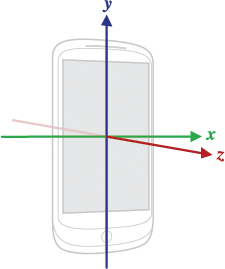
\includegraphics[scale=0.5]{images/axisDevice.png}
\captionof{figure}{The 3 principal axes of smartphones, defined with respect to the screen in its `natural orientation'~\cite{axisDevice}}
\label{fig:axisDevice}
\end{center}

As seen from the figure, the X-axis passes through the side of the phone, the Y-axis is along the vertical segment while the Z-axis projects out from the center of the screen. The positions of these axes remain fixed with respect to the screen, and thus rotate accordingly along with change in the phone's orientation. 


In order to confirm that the actual sensor readings correspond to the described behaviour the logging application was made use of in order to record and analyse the accelerometer data. The first recording was performed with the phone remaining stationary throughout and kept flat on the surface with the screen facing upwards. The readings obtained are shown in Figure~\ref{fig:accelerationZ}.

\begin{center}
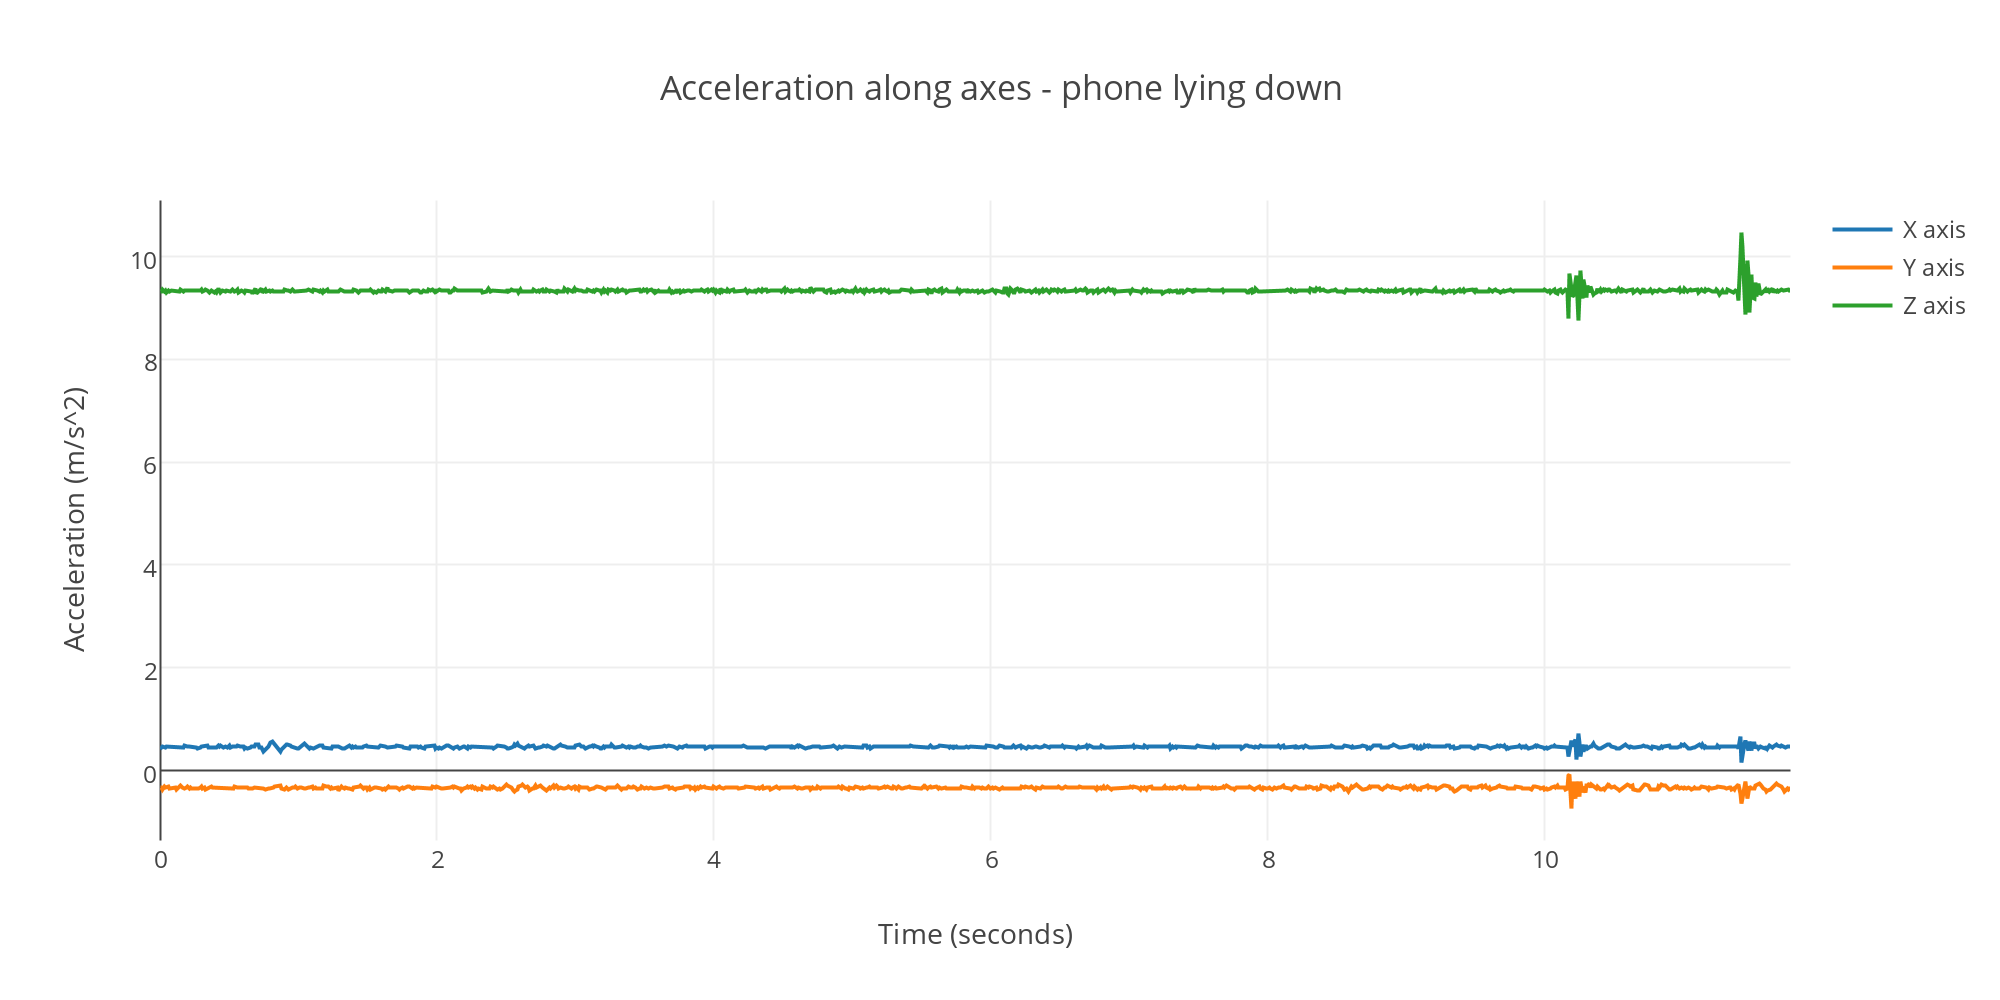
\includegraphics[scale=0.9]{images/accelerationZ.png}
\captionof{figure}{Accelerometer readings with phone kept flat on the surface}
\label{fig:accelerationZ}
\end{center}

As expected, the acceleration along the X and Y axes are close to 0, while there is a constant acceleration of about $9.81 m/s^2$ along the Z axis due to the force of gravity acting downwards through the screen of the phone. Note that the direction of acceleration in this case is upwards as the phone at rest accelerates upwards with respect to the local reference frame of a freely falling object close to the surface. 

This process is repeated with the phone held upright this time (with the bottom of the phone in contact with the surface). The obtained readings are shown in Figure~\ref{fig:accelerationY}.

\begin{center}
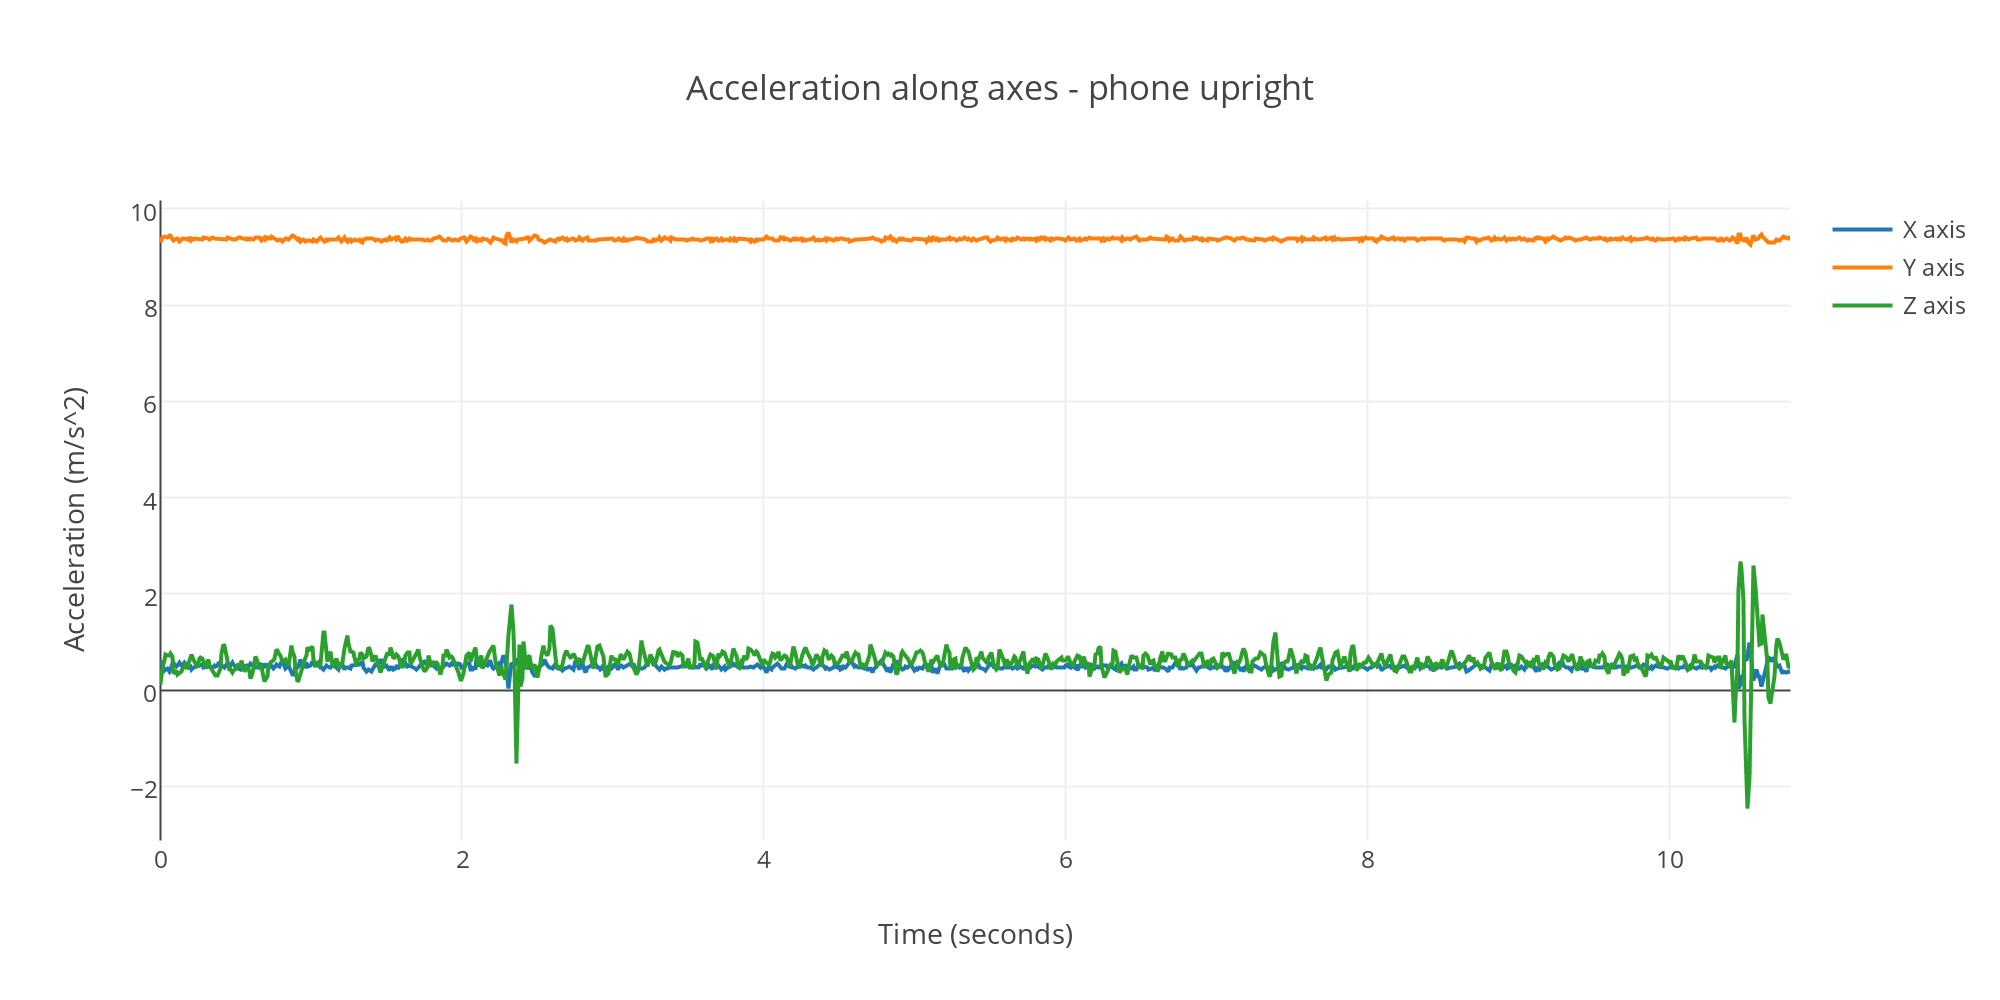
\includegraphics[scale=0.9]{images/accelerationY.png}
\captionof{figure}{Accelerometer readings with phone kept upright}
\label{fig:accelerationY}
\end{center}

The acceleration due to gravity is now along the Y-axis in accordance with the described behaviour, with the momentary spike in the Z-axis acceleration towards the end occurring due to slight movement of the hand while keeping the phone upright. On this basis it can also be concluded that keeping the phone lying on its side would make the gravity acceleration act along the X-axis, showing that the readings are consistent with the manner in which the phone's principal axes are defined. 
\\
\\
In addition to the accelerometer some approaches also consider the readings from the gyroscope, which is a sensor that measures the rate of rotation around the phone's principal axes~\cite{accelerometerAcceleration}. Such rotations can be correlated with the user's steps in certain situations, such as when the phone swings while the user has their hand to the side of their body while walking. However since this project restricts the phone's position to be in the user's hand and in front of them at all times there will be no considerable rotational motion involved. Thus the gyroscope readings will not provide any meaningful information for step detection and they are not considered in our approach. 

\section*{Initial Data Analysis}

After deciding that the accelerometer readings would form the basis of the step detection approach, the logging application was used to capture some acceleration data corresponding to walking motion to perform an initial analysis and detect any patterns that could be associated with individual steps. The data was recorded while keeping the phone in hand and walking in a straight line for approximately 10 steps. 
The obtained data is depicted in Figure~\ref{fig:straightWalkRaw}. 

\begin{center}
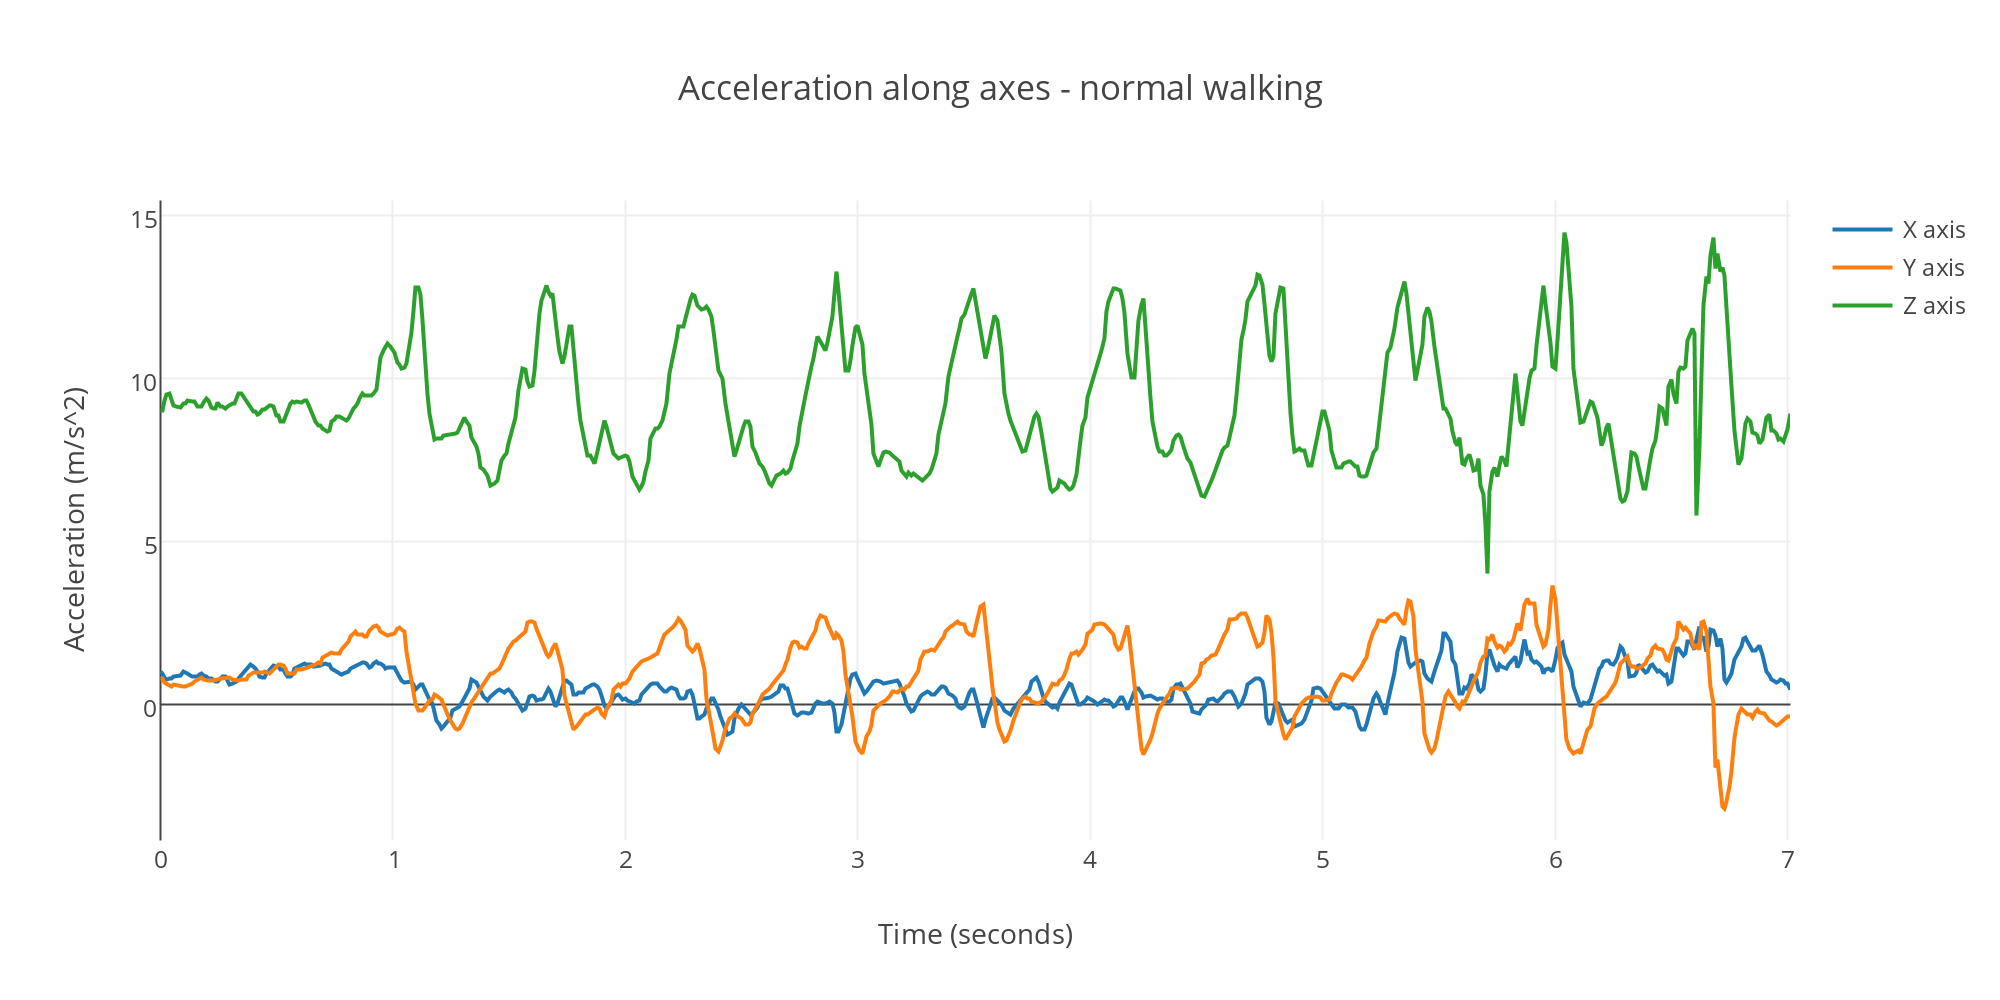
\includegraphics[scale=0.9]{images/straightWalkRaw.png}
\captionof{figure}{Accelerometer readings during normal walking}
\label{fig:straightWalkRaw}
\end{center}

As observed in the figure there is a periodic rise and fall in both the Y-axis and Z-axis accelerometer readings, while the X-axis readings do not exhibit much variation and remain close to 0 throughout. This is because when the phone is kept in the hand in portrait mode the majority of the gravity component is split vertically among the Y and Z axes, while there is negligible horizontal acceleration.

The periodicity in the Y and Z readings corresponds to the two phases of walking motion - the user beginning their step by lifting their foot off the surface followed by completing the step with bringing their foot down to make contact with the surface again. The first phase causes the phone to accelerate vertically along the direction of gravity acceleration as the user moves upwards. These are represented as peaks in the graph as the accelerations add together. In the second phase the user moves downwards and thus accelerates in a direction opposite to that of the gravity acceleration, leading to the formation of the valleys in the graph. Thus each peak/valley combination can be associated with individual steps, potentially allowing step identification to be carried out by detecting peaks and valleys in the graph generated by the accelerometer readings. This notion is supported by the plot in Figure~\ref{fig:straightWalkRaw}, where there are roughly 10 peak/valley pairs for both the Y and Z readings corresponding to the 10 steps taken.   

The primary issue with this approach is that step detection is dependent on the orientation in which the phone is kept. For instance, if the user holds the phone in landscape mode instead of portrait then a major component of the acceleration will  be along the X axis. This makes it difficult to keep track of periodic changes in acceleration as variations along all the three axes must be considered simultaneously depending on the phone's orientation. This problem is overcome by computing the magnitude of the accelerometer vector and using that instead to detect steps. The magnitude combines the acceleration information from the three axes into a single scalar quantity, which by definition, is independent of direction and makes it robust to changes in orientation. The magnitude plot of the acceleration values in Figure~\ref{fig:straightWalkRaw} is provided in Figure~\ref{fig:straightWalkRawMagnitude}. 

\begin{center}
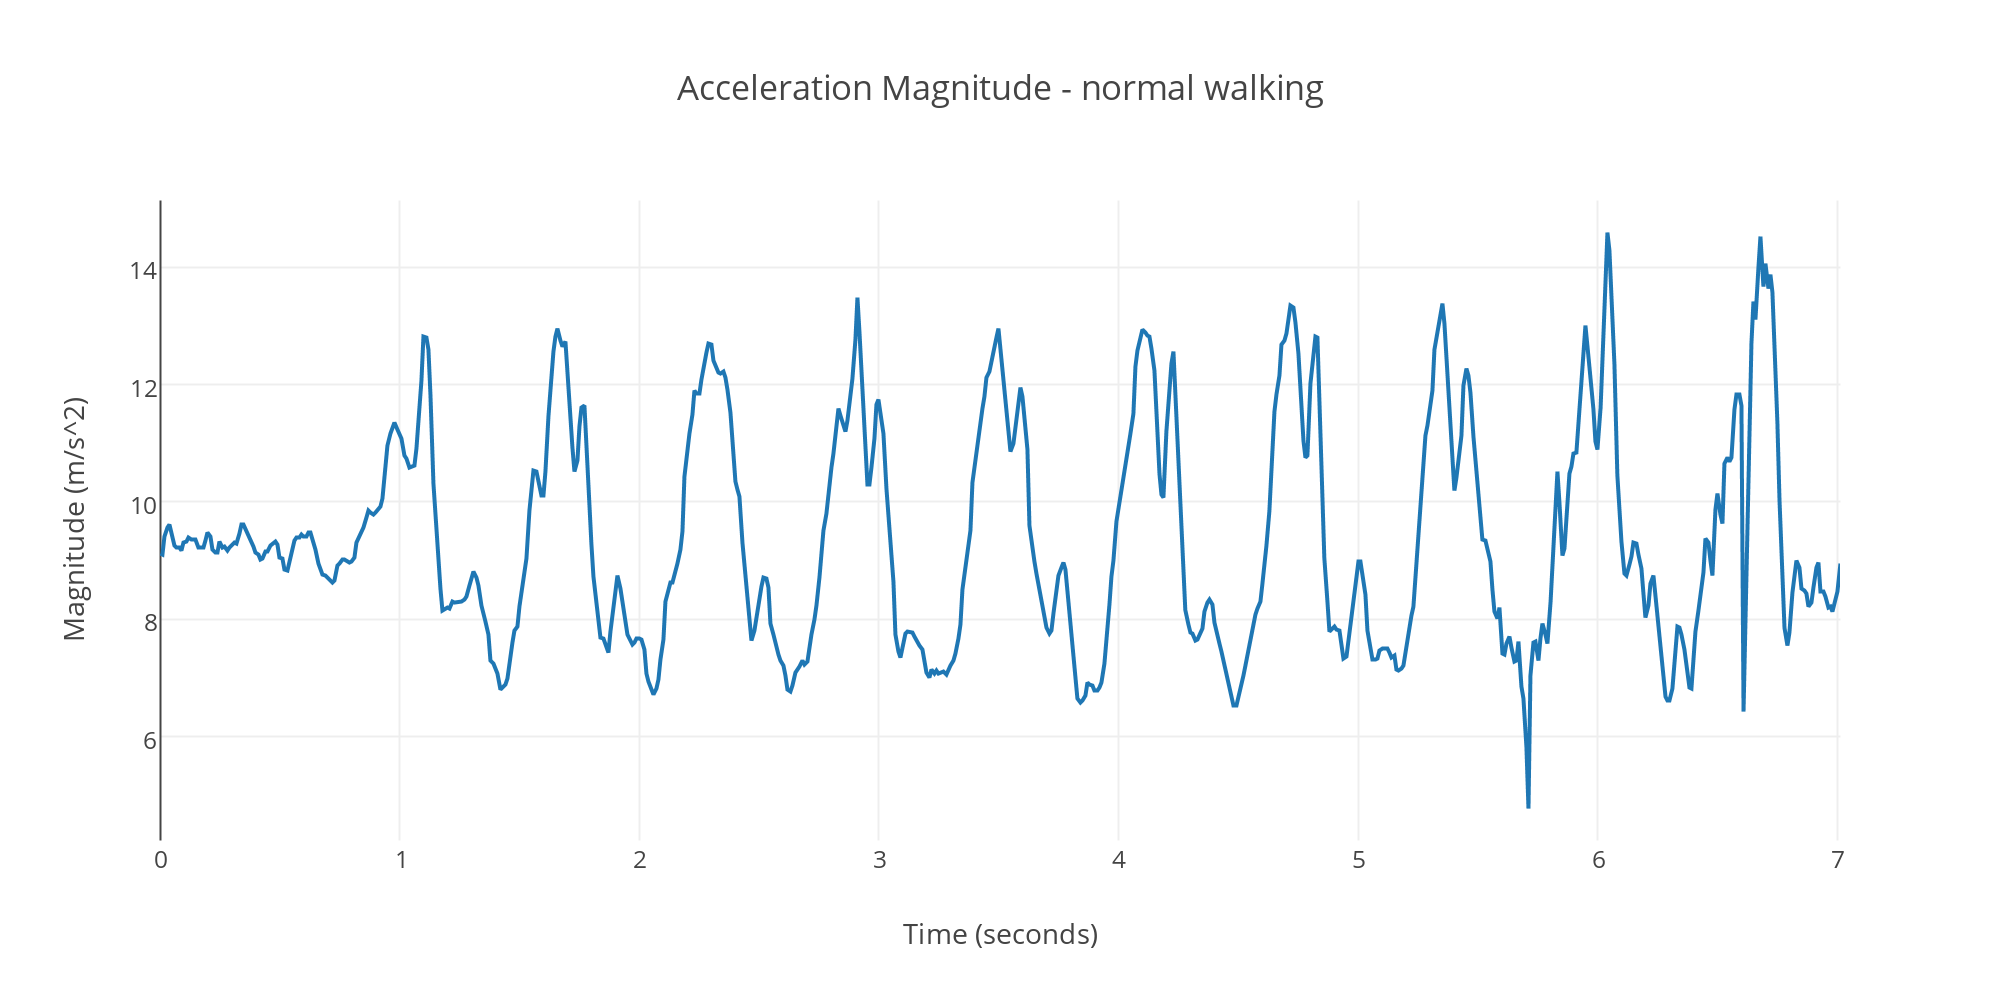
\includegraphics[scale=0.9]{images/straightWalkRawMagnitude.png}
\captionof{figure}{Accelerometer magnitude during normal walking}
\label{fig:straightWalkRawMagnitude}
\end{center}

From the plot it can be seen that using magnitude still preserves the 10 peak/valley pairs corresponding to steps that were identified in the previous graph. Thus step detection can now be carried out on the basis of a single measure that accounts for changes in orientation. 

\section*{Peak/valley detection}

Figures~\ref{fig:straightWalkRaw} and~\ref{fig:straightWalkRawMagnitude} show a clear association between steps taken and peak/valley pairs in the graph. Thus individual steps can be identified by detecting the formation of such pairs in real-time. Mathematically, peaks are defined as points in the graph where the slope transitions from positive to negative. Equation~\ref{eq:peakDetection} shows how it can be determined whether a point is a peak. 

\begin{equation}\label{eq:peakDetection}
\begin{split}
previousSlope = a(n) - a(n-1) \\
newSlope = a(n+1) - a(n) \\
a(n) = peak\ if\ previousSlope > 0\ \&\ newSlope < 0
\end{split}
\end{equation}
where $a(n)$ is the $n$th reading from the accelerometer. Similarly, valleys are defined as points where the slope transitions from negative to positive. Equation~\ref{eq:valleyDetection} gives the criteria for a point to be classified as a valley. 

\begin{equation}\label{eq:valleyDetection}
a(n) = valley\ if\ previousSlope < 0\ \&\ newSlope > 0
\end{equation}
In the application, each new reading from the accelerometer is checked to see whether it is a peak or valley. This is done by maintaining a small sliding window of the three most recent accelerometer values. The middle value in this window is the one which is subject to the peak/valley check as the required slopes can be computed from the adjacent values. A step event is thus fired whenever a valley and peak are detected in succession.  

On applying this step detection approach to the graph in Figure~\ref{fig:straightWalkRawMagnitude} it is found that the number steps returned by the algorithm is significantly greater than the actual number of steps that were taken. This is due to the jagged nature of the graph, which is a consequence of the phone's accelerometer having high sensitivity. Even very slight movements cause non-negligible acceleration to be recorded, which leads to the introduction of a considerable amount of noise arising from the jitters and vibrations experienced by the phone while walking. These jitters result in a number of small kinks in the accelerometer graph that are interpreted as peaks/valleys by the step detector, triggering false positives. There is thus a need to remove these kinks by applying some smoothing so that only large changes in acceleration cause peaks and valleys to be formed.  

\section*{Low-pass filtering}

A low-pass filter is a filter which allows low frequency signals to pass through while attenuating signals that are above a defined `cut-off frequency'. In essence, it smooths the signal by eliminating small, momentary fluctuations while preserving any significant changes in the signal that occur gradually over a longer period. Hence a low-pass filter is applied to the accelerometer readings in order to counteract the effects of the added noise and remove the kinks in the graph which contribute to false positives, while resulting in the peaks and valleys corresponding to steps taken to be more well defined. 

\subsection*{Exponential smoothing}

The simplest type of low-pass filter is a first order one. The order of a filter refers to how sharply it reduces the amplitude of a signal whenever its frequency doubles. For instance, a first order filter halves the signal's amplitude while higher orders cause greater reductions~\cite[p.2528]{casiez20121}. A simple digital implementation of a first order low-pass filter is given in Equation~\ref{eq:lowPass}.   

\begin{equation}\label{eq:lowPass}
\hat{a}(n) = \alpha \times a(n) + (1 - \alpha) \times \hat{a}(n-1)
\end{equation}
where $\hat{a}(n)$ is the $n$th filtered accelerometer value, and $\alpha$ is a constant, known as the smoothing factor, between 0 and 1. Lower values of $\alpha$ (say 0.25) mean that each new filtered value is computed by taking a large proportion of the previous filter output and providing a slight update to it using the most recent raw accelerometer reading. This is represented diagrammatically in Figure~\ref{fig:complementaryFilter}.  

\begin{center}
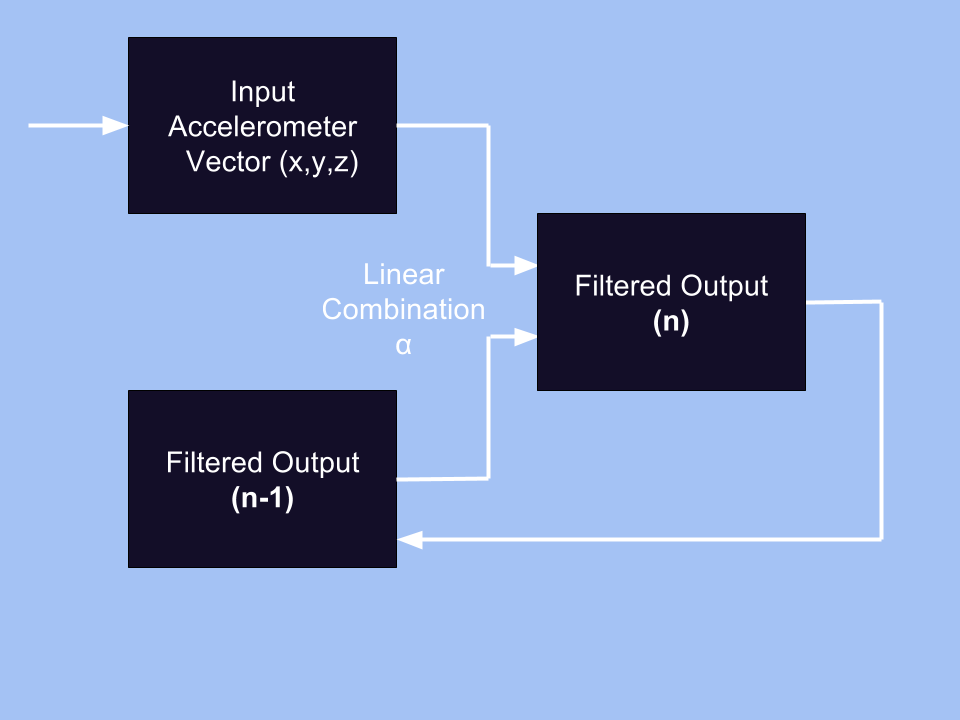
\includegraphics[scale=0.3]{images/complementaryFilter.png}
\captionof{figure}{First order low-pass filter for accelerometer readings}
\label{fig:complementaryFilter}
\end{center}
Thus any variations in the raw input values must occur consistently over a sustained time period for it to be reflected in the filtered output. This process is known as `exponential smoothing' since ``the contribution of the older values exponentially decreases'' over time~\cite[p.2528]{casiez20121}. The result of applying this filter on the magnitude values in Figure~\ref{fig:straightWalkRawMagnitude} is shown in Figure~\ref{fig:complementaryFilterMagnitude}. 

\begin{center}
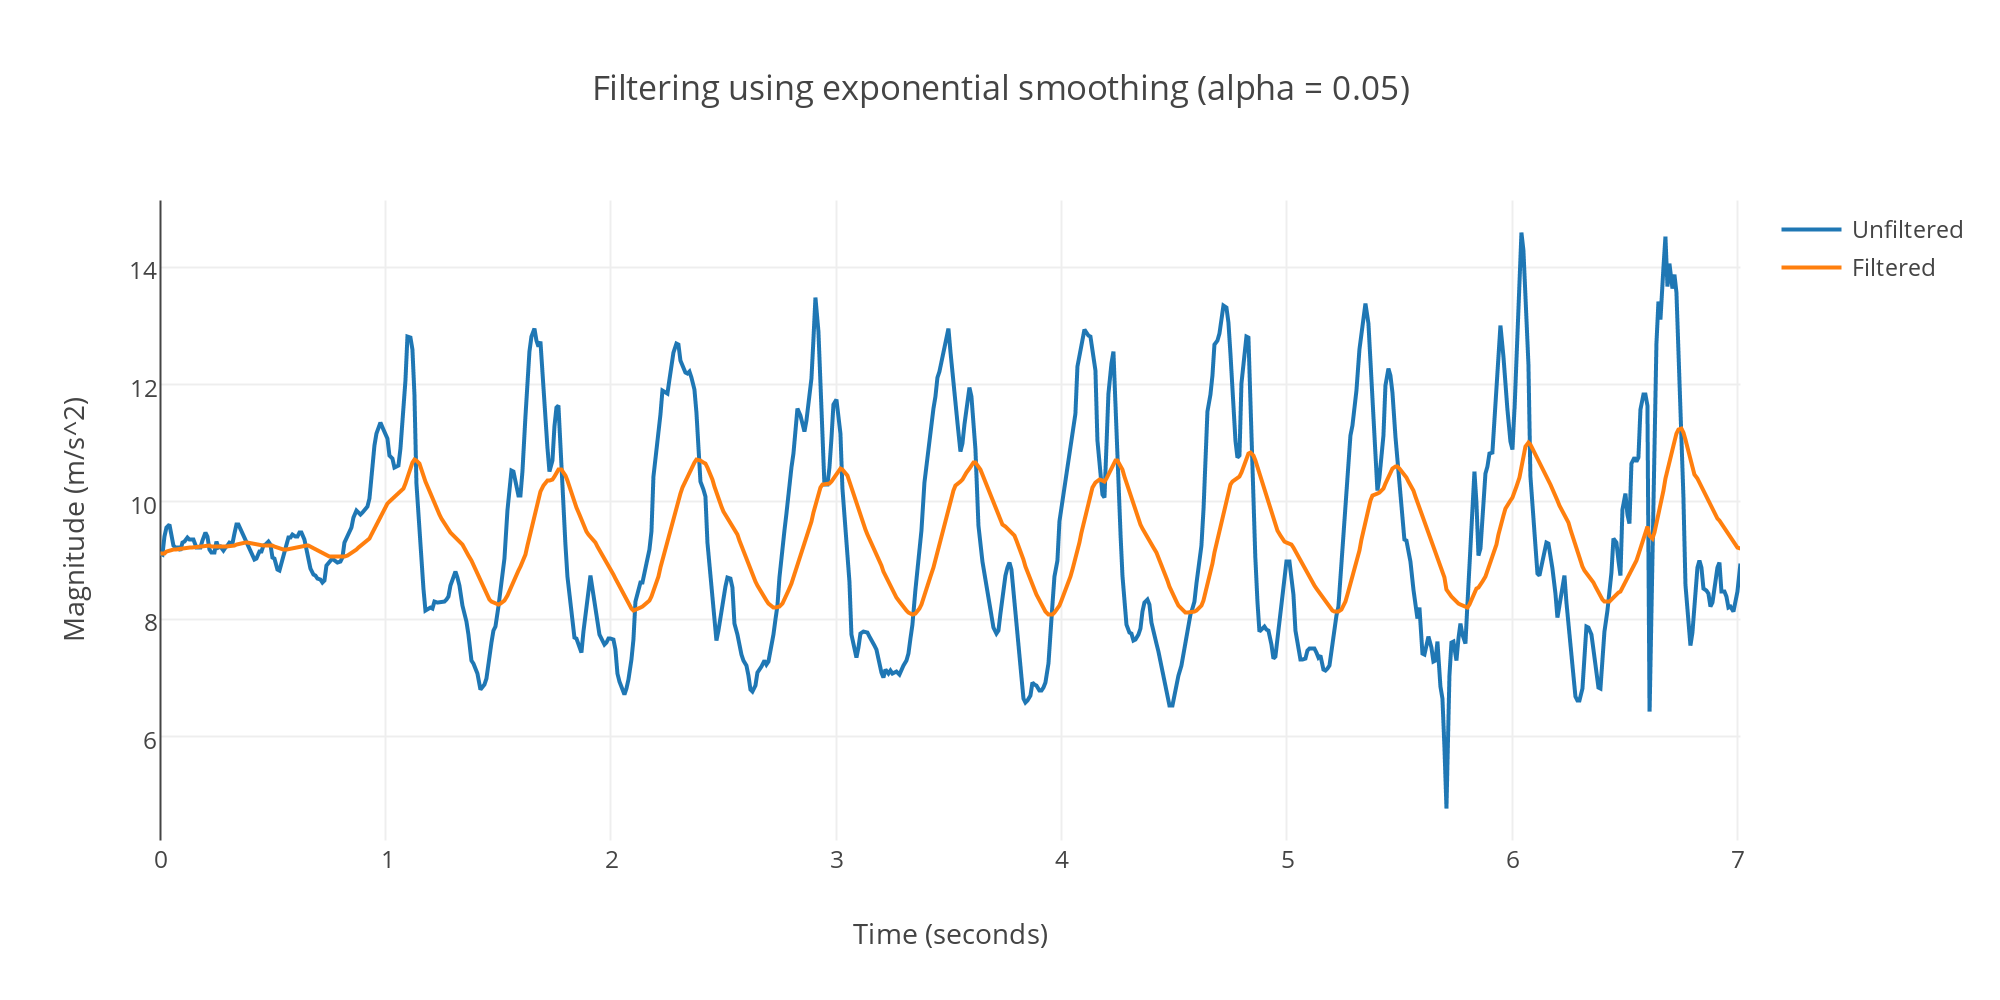
\includegraphics[scale=0.9]{images/complementaryFilterMagnitude.png}
\captionof{figure}{Result of applying exponential smoothing to the unfiltered magnitude}
\label{fig:complementaryFilterMagnitude}
\end{center}

The filtered graph obtained is far smoother than its unfiltered counterpart and removes most of its kinks, thus reducing the number of false positives with regards to step detection.   

On initial tests using this approach the step counting was found to be fairly accurate during standard walking motion, with each individual step being detected almost immediately after it was actually taken. However, step events were also often found to fire when the user was stationary and performing other activities while having the phone in their hand. For instance, it was observed that modest hand motions of the user while standing and talking to someone resulted in steps being recorded. This suggests that the accelerometer magnitude patterns produced by such motions are similar to those obtained while walking. In order to investigate this the logging application was used to record accelerometer values while the phone was kept in hand and moved up and down slightly in a periodic manner without taking any steps. The filtered output from this recording is shown in Figure~\ref{fig:complementaryFilterHandMotionMagnitude}. 

\begin{center}
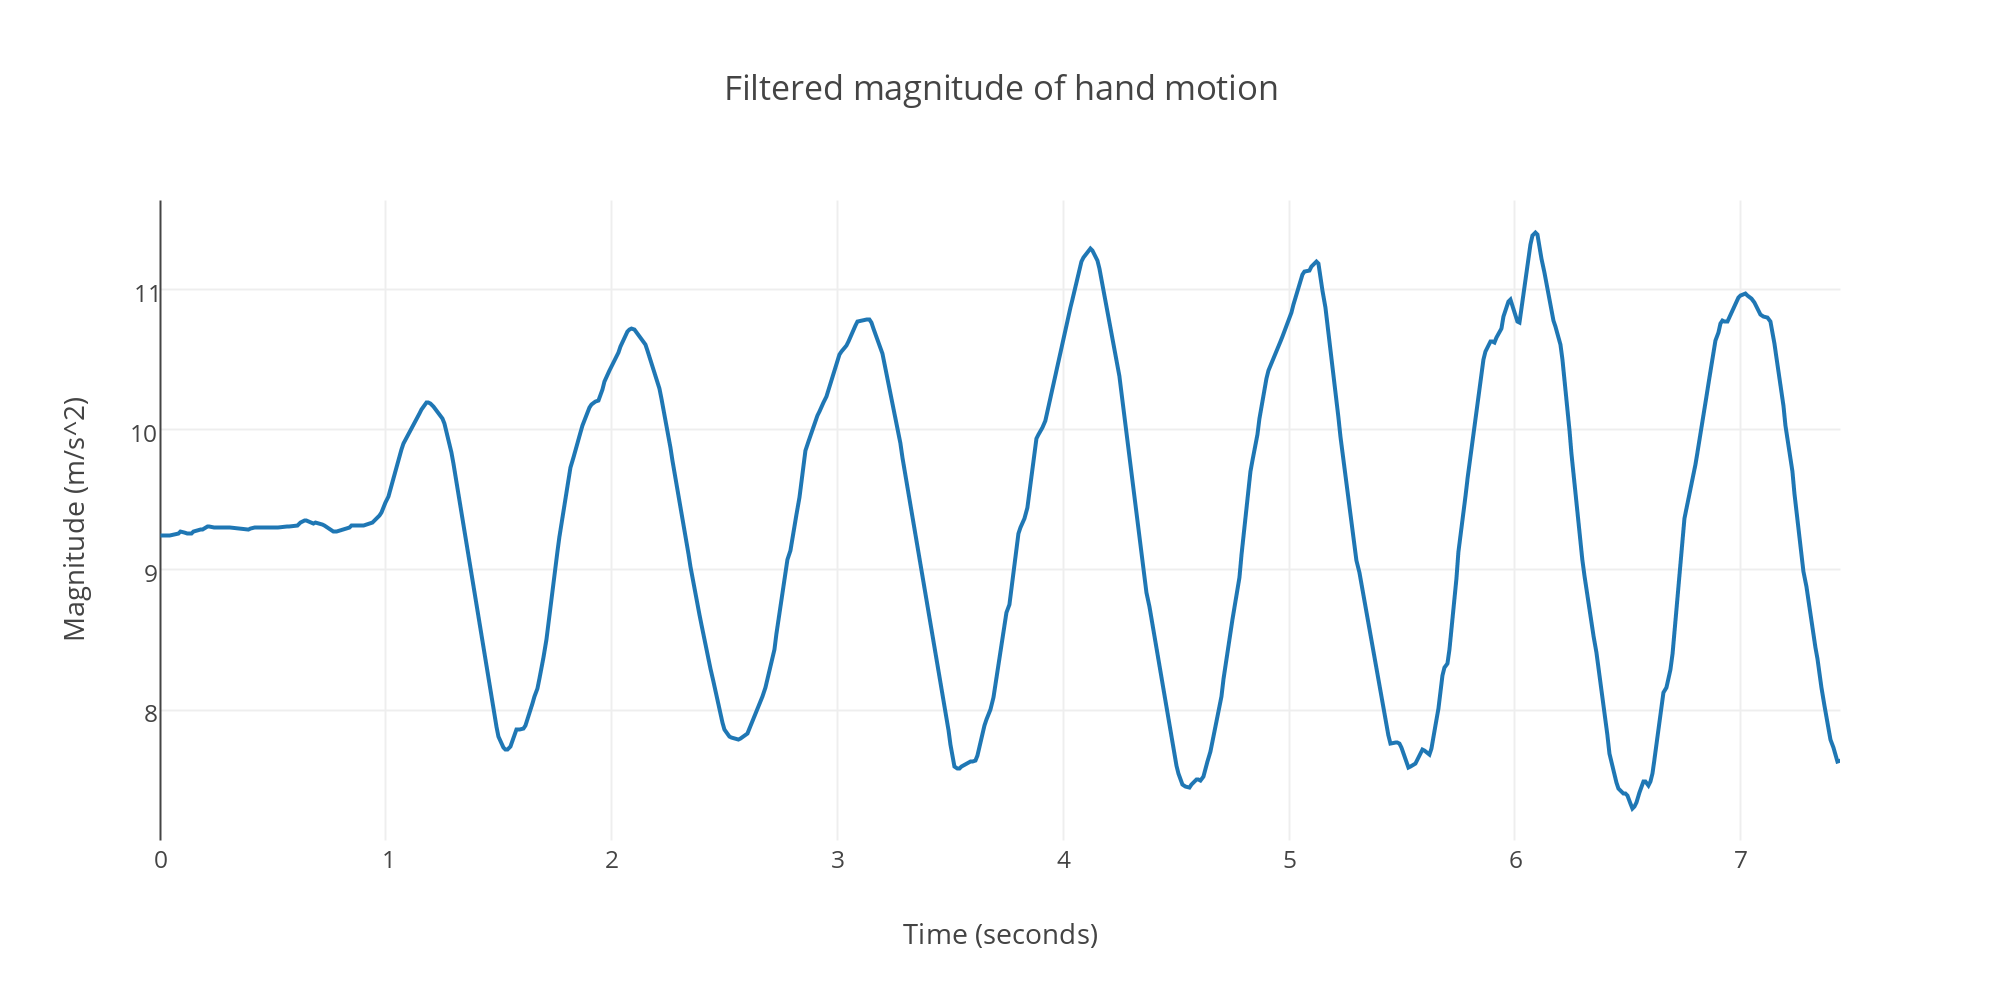
\includegraphics[scale=0.9]{images/complementaryFilterHandMotionMagnitude.png}
\captionof{figure}{Filtered magnitude of hand motion}
\label{fig:complementaryFilterHandMotionMagnitude}
\end{center}
The plot confirms that using the exponential smoothing method to filter these hand motions produces peak/valley combinations that are almost indistinguishable from normal walking motion and results in steps being detected falsely. This first-order filter is thus deemed to be too sensitive for the purpose of navigation. 

\subsection*{Butterworth Filter}

A `Butterworth' low-pass filter is one that is mathematically designed to provide as flat a frequency response as possible in the passband while dropping off towards zero in the stopband~\cite[p.17]{bianchi2007electronic}. This means that in the ideal scenario, components of the signal below the cut-off frequency are passed through at maximum amplitude without any ripples while high frequency components are eliminated through attenuation. This is depicted in Figure~\ref{fig:butterworthResponse}.   

\begin{center}
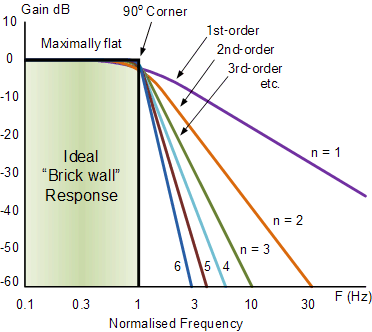
\includegraphics[scale=0.9]{images/butterworthResponse.png}
\captionof{figure}{Plot of gain vs normalised frequency for various Butterworth filter orders~\cite{butterworthResponse}}
\label{fig:butterworthResponse}
\end{center}
The 'brick wall' response represents the ideal case with the steepest possible 90 degree corner passband, where the amplitude of any signal greater than the cut-off frequency immediately drops to zero. For practical purposes however, it is only possible to obtain approximations for this ideal Butterworth response as maximal steepness produces significant passband ripple~\cite{butterworthResponse}. 

Using an approximation of this ideal response means that a flat passband can be achieved only by introducing a `transition band', the range of frequencies between the passband and stopband for which the amplitude is neither maximum nor zero. From the figure it can be seen that first-order filters have a very wide transition band, meaning that only signals that have considerably greater frequency than the cut-off are fully attenuated. Filters of greater order cause more aggressive attenuation, which is why increasing the order of the Butterworth filter leads to a better approximation of the ideal response as shown in the diagram. Thus using a high order Butterworth filter provides good separation between the passband and stopband while minimising the interference caused to the signal in the passband due to ripples.    

Mathie, M. analysed the manner in which readings from a triaxial accelerometer could be used to detect and classify a wide variety of human movements and actions. As part of this research, they found that the frequency range of 0.7-3 Hz encompasses most people's normal walking motions~\cite[p.248]{walkingFrequency}. This is derived from the total number of steps usually taken per minute while walking. Hence using a low-pass Butterworth filter with a 3 Hz cut-off frequency would allow isolation of the accelerometer signals associated with walking motion while removing any potential higher frequency components introduced by noise and other external factors. For instance, Susi, M., et al. employ a tenth-order Butterworth filter for pre-processing the accelerometer readings to make their step detection algorithm robust to such high frequency signals~\cite[p.1552]{susi2013motion}.  

With this in mind we too tried using the same tenth-order Butterworth filter in order to see whether it would improve step detection performance in comparison to the first-order exponential smoothing approach. This filter was implemented by using an online tool provided by Fisher, T., a professor at the University of York~\cite{filterTool}, which takes user-specified input parameters such as the desired cut-off frequency and filter order to generate the corresponding recursive Butterworth filter equation. The 3 Hz, tenth-order filter obtained computes each new filtered value on the basis of the 11 latest raw input values and 10 previous filter output values. The results of applying this filter on the normal walking and hand motion accelerometer readings are depicted in Figure~\ref{fig:butterworth10thOrderFilter}. 
\begin{center}
  \begin{minipage}[b]{0.5\textwidth}
    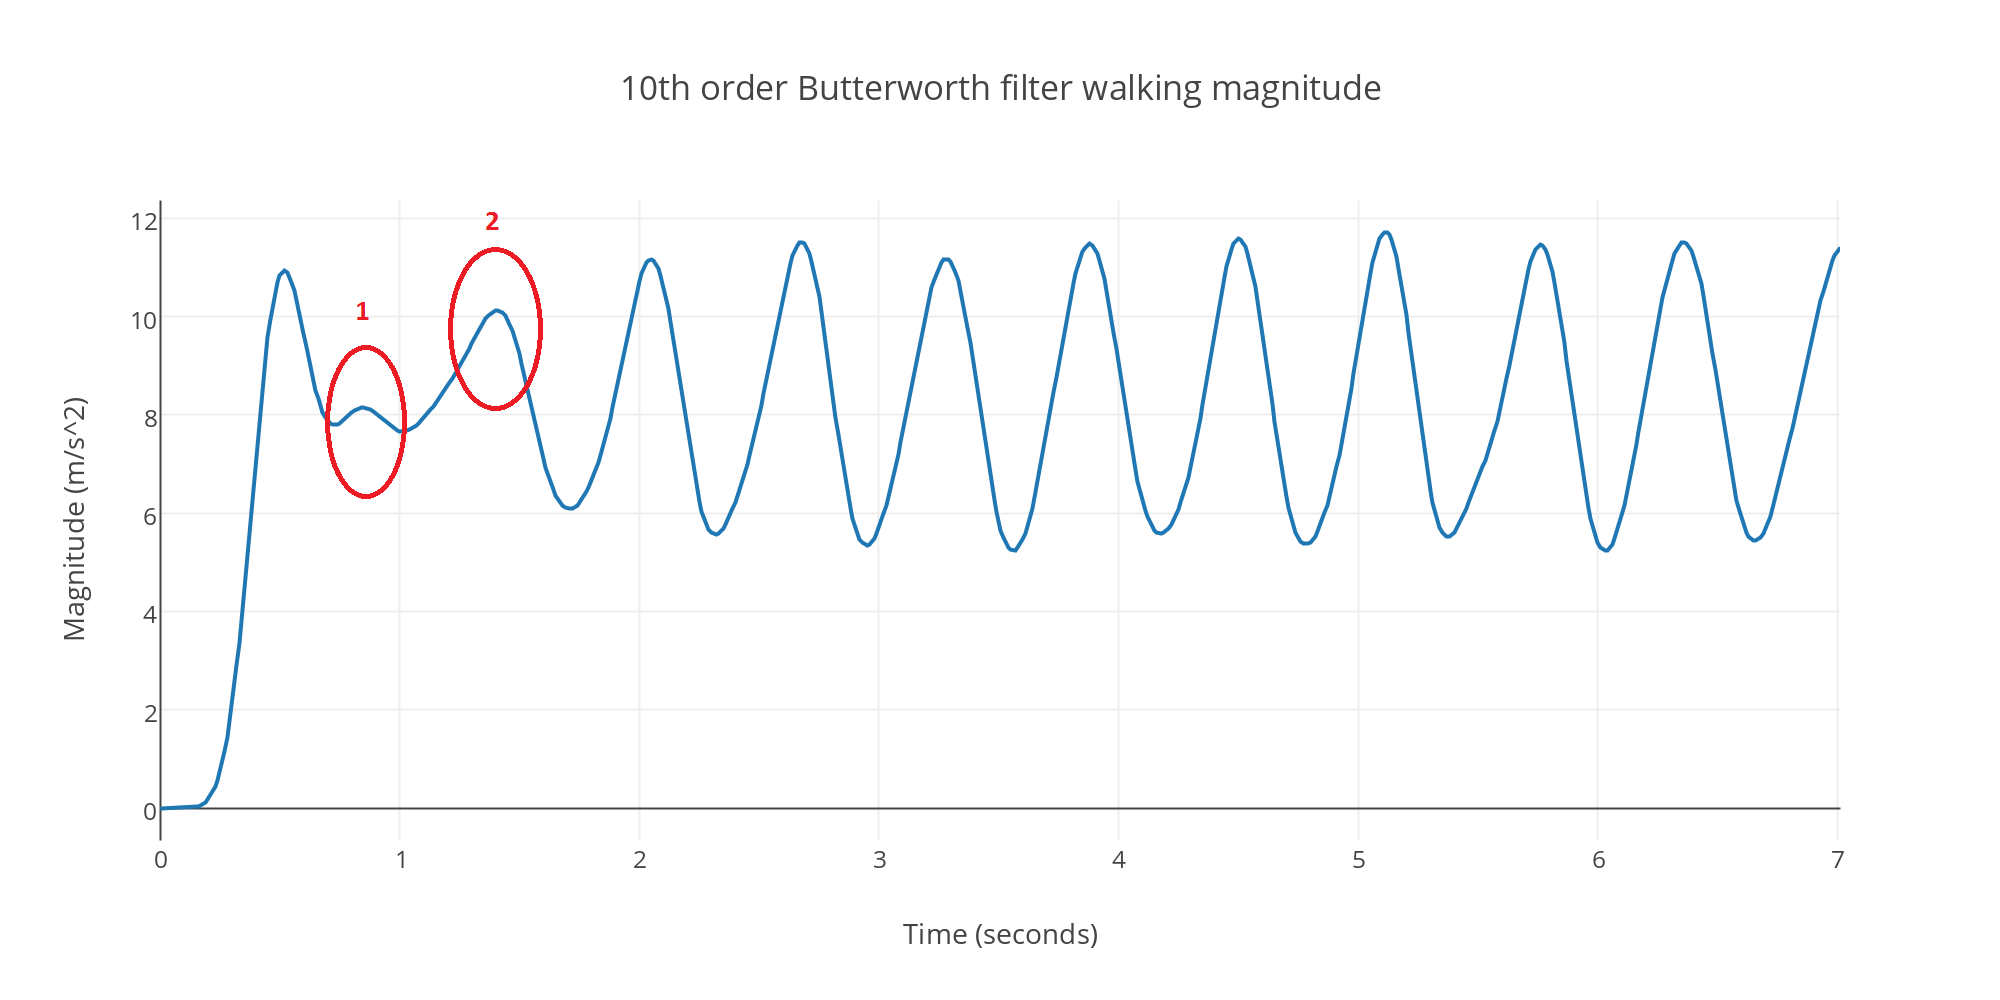
\includegraphics[scale=0.2]{images/butterworth10thOrderFilterWalkingMagnitude.png}
  \end{minipage}%
  \begin{minipage}[b]{0.5\textwidth}
    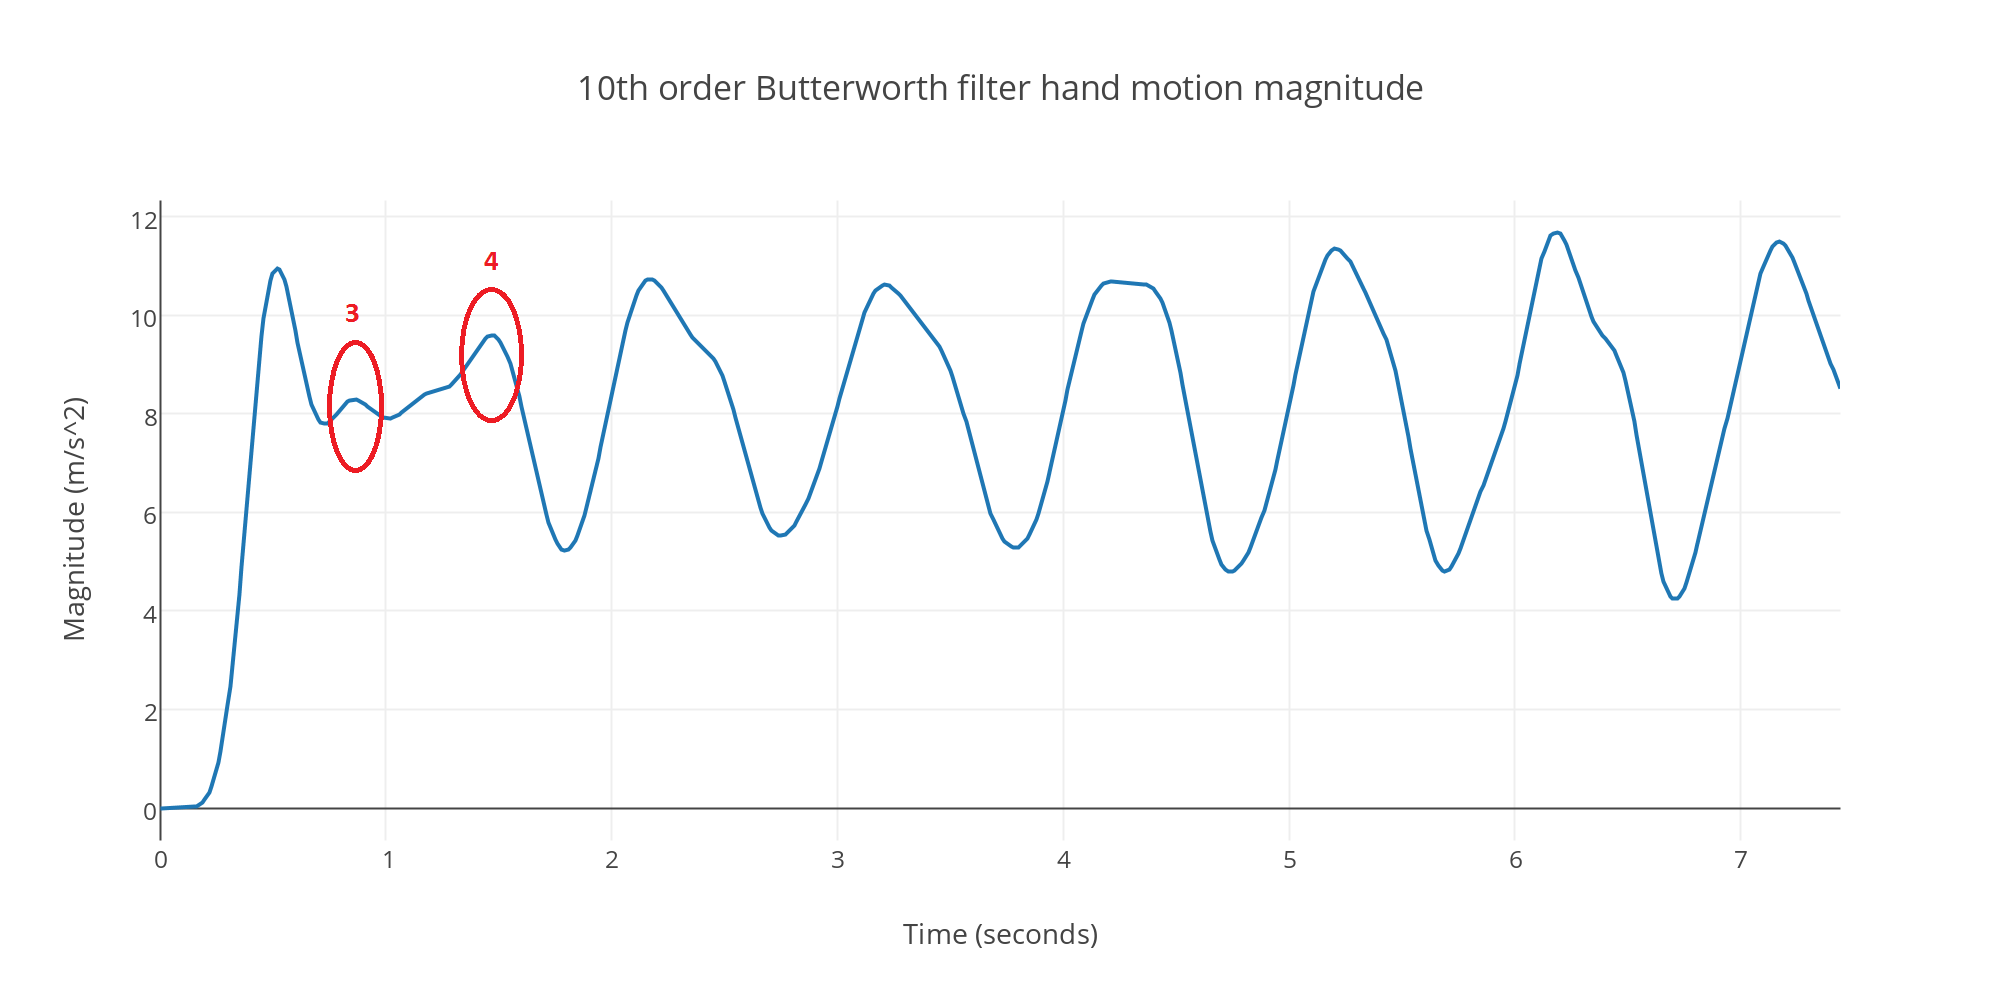
\includegraphics[scale=0.2]{images/butterworth10thOrderFilterHandMotionMagnitude.png}
\end{minipage}
\captionof{figure}{Results of applying the tenth-order Butterworth filter}
\label{fig:butterworth10thOrderFilter}
\end{center}
On initial inspection it seems that the filtered graphs obtained for both walking and hand motion are once again similar, just like they were for the first-order filter. However, there exists a significant difference between the two filters with regards to the magnitudes of the peaks/valleys obtained. In both the plots in Figure~\ref{fig:butterworth10thOrderFilter} the first peak is formed due to the initial adjustment of the filter as it shifts from its initial value of zero to the new magnitude values coming in, and hence this peak can be ignored for the purpose of step detection. The following two peaks in each plot, denoted by the numbers 1/2 and 3/4 respectively, have magnitude values that are noticeably lower than those of the subsequent peaks. Furthermore, the magnitude values of these subsequent peaks and valleys are largely consistent, that is, the peaks and valleys occur at almost the same magnitude values in all cases. Thus there is a clear differentiation between the first two peaks and the following ones. This is in contrast to the plots obtained when using the first-order filter (Figures~\ref{fig:complementaryFilterMagnitude} and~\ref{fig:complementaryFilterHandMotionMagnitude}) where all the peaks, including the first two, have similar magnitude values. 

The variation in behaviour between the two filters occurs due to them having different orders. As shown in Equation~\ref{eq:lowPass}, the first-order filter computes new filtered values only on the basis of the single latest raw input and the single previous filter output. In comparison, the tenth-order Butterworth filter makes use of a much larger `history' of values (11 input and 10 output values). This means that any changes in the raw input values are initially reflected more prominently in the first-order filter since the history of previous values before the change in case of the tenth-order filter result in a relatively smaller change in its output. This is the reason why the first two peaks in the accelerometer outputs of the tenth-order filter have relatively lower magnitudes as the history of values `catch up' to the variation in acceleration during walking after the preceding constant acceleration when starting from a stationary position. These variations are fully reflected in the output for the subsequent peaks as the change in input occurs periodically over a sustained interval. 

It is this difference in the magnitudes of the initial peaks between the exponential smoothing and Butterworth filter approaches which enables the latter to detect false step positives arising from the user's hand motions. Not accounting for the case where the user attempts to `cheat' the step detector by moving the phone up and down periodically in a contrived manner so as to match the frequency at which steps are taken, the occasional user hand motions encountered during navigation are expected to be short, momentary jerks rather than sustained actions. In contrast, regular walking is a motion that occurs consistently over a larger interval. Thus the filtered acceleration peaks produced by the hand motions will be few in number and have relatively small magnitudes whereas walking motion will eventually produce peaks of higher magnitudes consistently. By imposing a minimum threshold $t_{min}$ for the magnitude difference between a valley and a peak for that pair to be counted as a step, hand motion false positives can be avoided. An example of applying this process on the filtered walking motion graph is shown in Figure~\ref{fig:butterworth10thOrderFilterWalkingMagnitudeThreshold}. 

\begin{center}
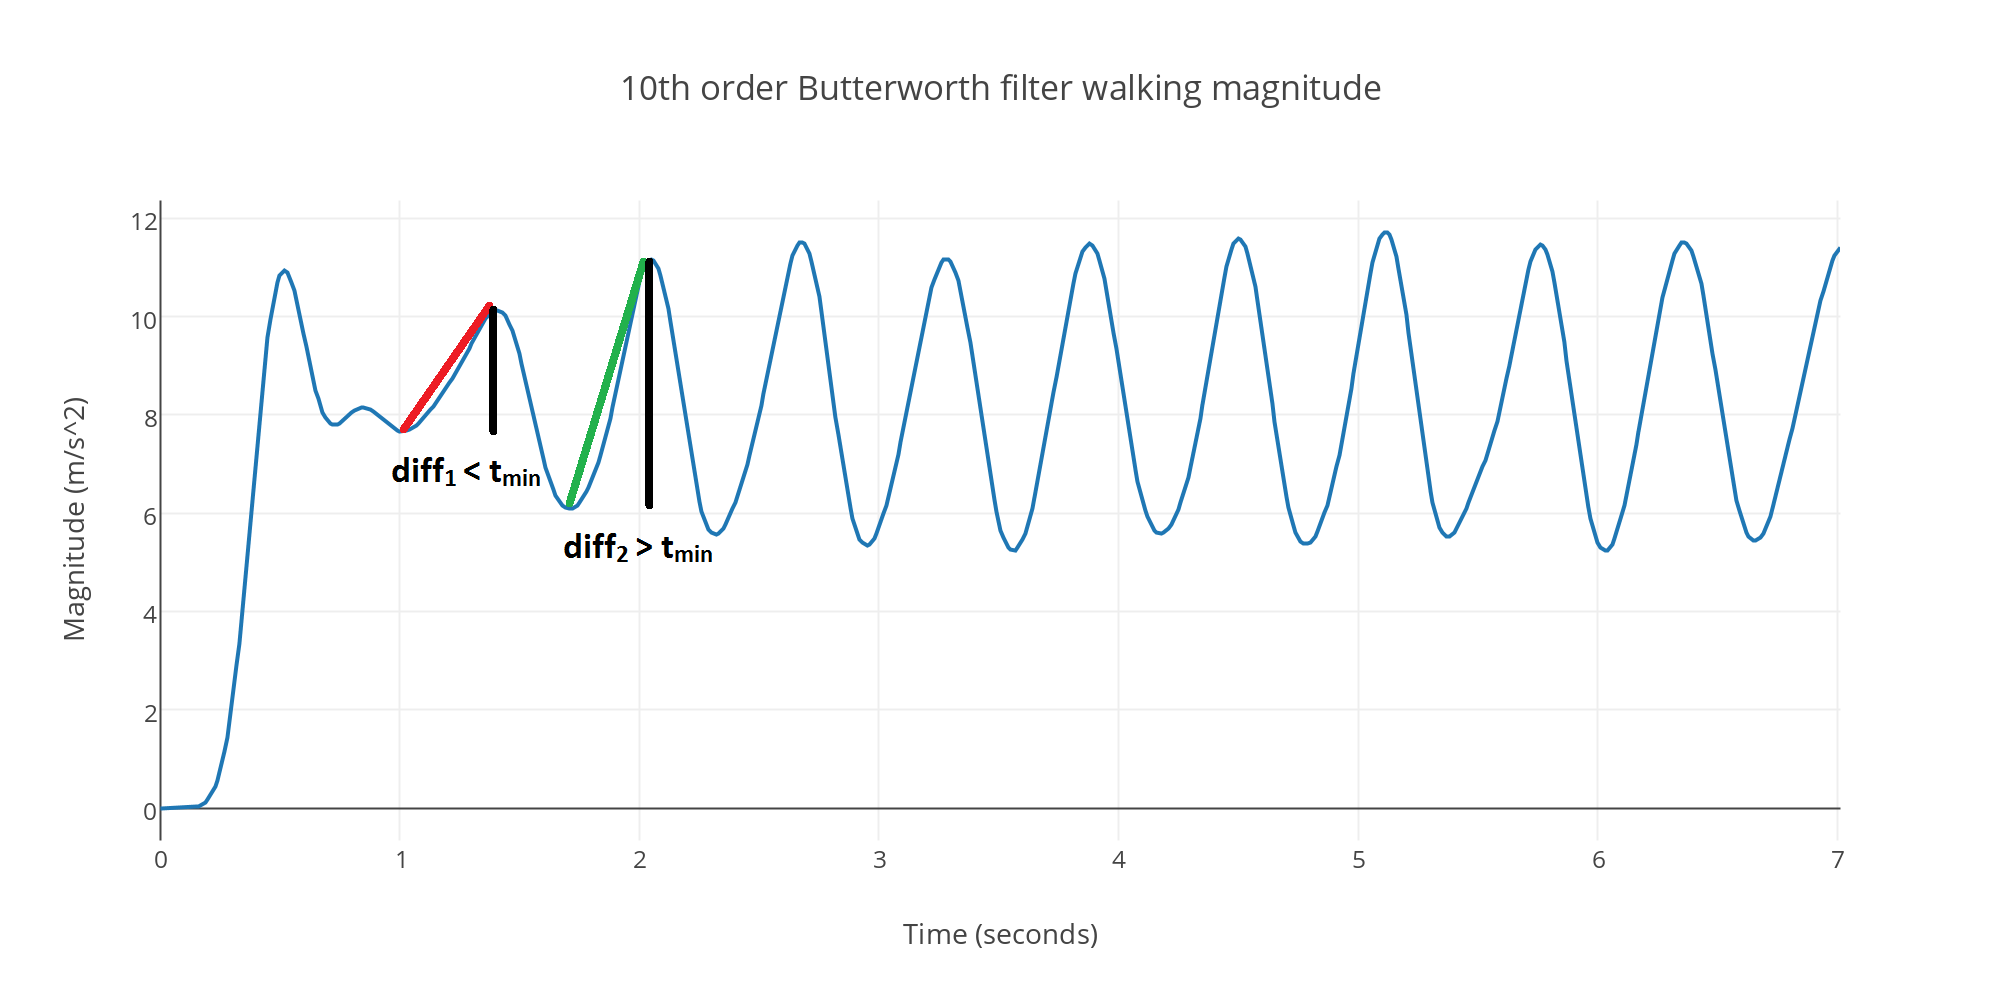
\includegraphics[scale=0.2]{images/butterworth10thOrderFilterWalkingMagnitudeThreshold.png}
\captionof{figure}{Applying minimum magnitude thresholding to avoid false positives}
\label{fig:butterworth10thOrderFilterWalkingMagnitudeThreshold}
\end{center}
In this case the magnitude difference between the second valley and second peak (not counting the first actual pair formed due to initial filter adjustment), represented by $\mathit{diff}_1$ in the graph, is below the minimum threshold $t_{min}$ and thus this pair does not trigger a step event. The magnitude difference $\mathit{diff}_2$ between the next valley and peak however is greater than $t_{min}$ and this counts as a step. For sudden hand motions, only the first 1-2 peaks will be produced in the filtered output and since both will ideally be below $t_{min}$ no false positives will be recorded. For standard walking, the first step will be recorded on the 3rd valley/peak combination in this instance. This approach also accounts for the previous `missed' pairs, which are actual legitimate steps in such cases, by keeping a record of valley/peak combinations that would have triggered a step but were below the threshold. Once the first step above $t_{min}$ has been detected the algorithm then knows that the previous peaks were not formed due to hand motions and counts those towards the step total as well. Note that a separate minimum threshold $t_{significant}$, which is smaller than $t_{min}$, is used to decide whether a valley/peak pair should be included in the record maintained. This ensures that very small peaks produced through slight sensor fluctuations rather than any actual motion are excluded.  

Initial tests with this approach showed that it was more robust with regards to false positives as compared to the first-order filter, with steps being recorded far less frequently for slight hand motions. However, with step detection during normal walking itself it was found that there was a noticeable lag between when steps were recorded and actually taken. This can once again be attributed to filter output computation being based on the large history of values, which results in any changes to the input being reflected a short while after they actually occur. As the first-order filter was deemed to be too sensitive and the tenth-order filter is too laggy, a fifth-order Butterworth filter, which uses 6 input and 5 filter output values, is used to attain the middle ground in the compromise between robustness and reactivity. The results of applying the fifth and tenth-order filters on the accelerometer readings for normal walking motion are compared in Figure~\ref{fig:butterworth5thVs10thOrderWalkingMagnitude}.  

\begin{center}
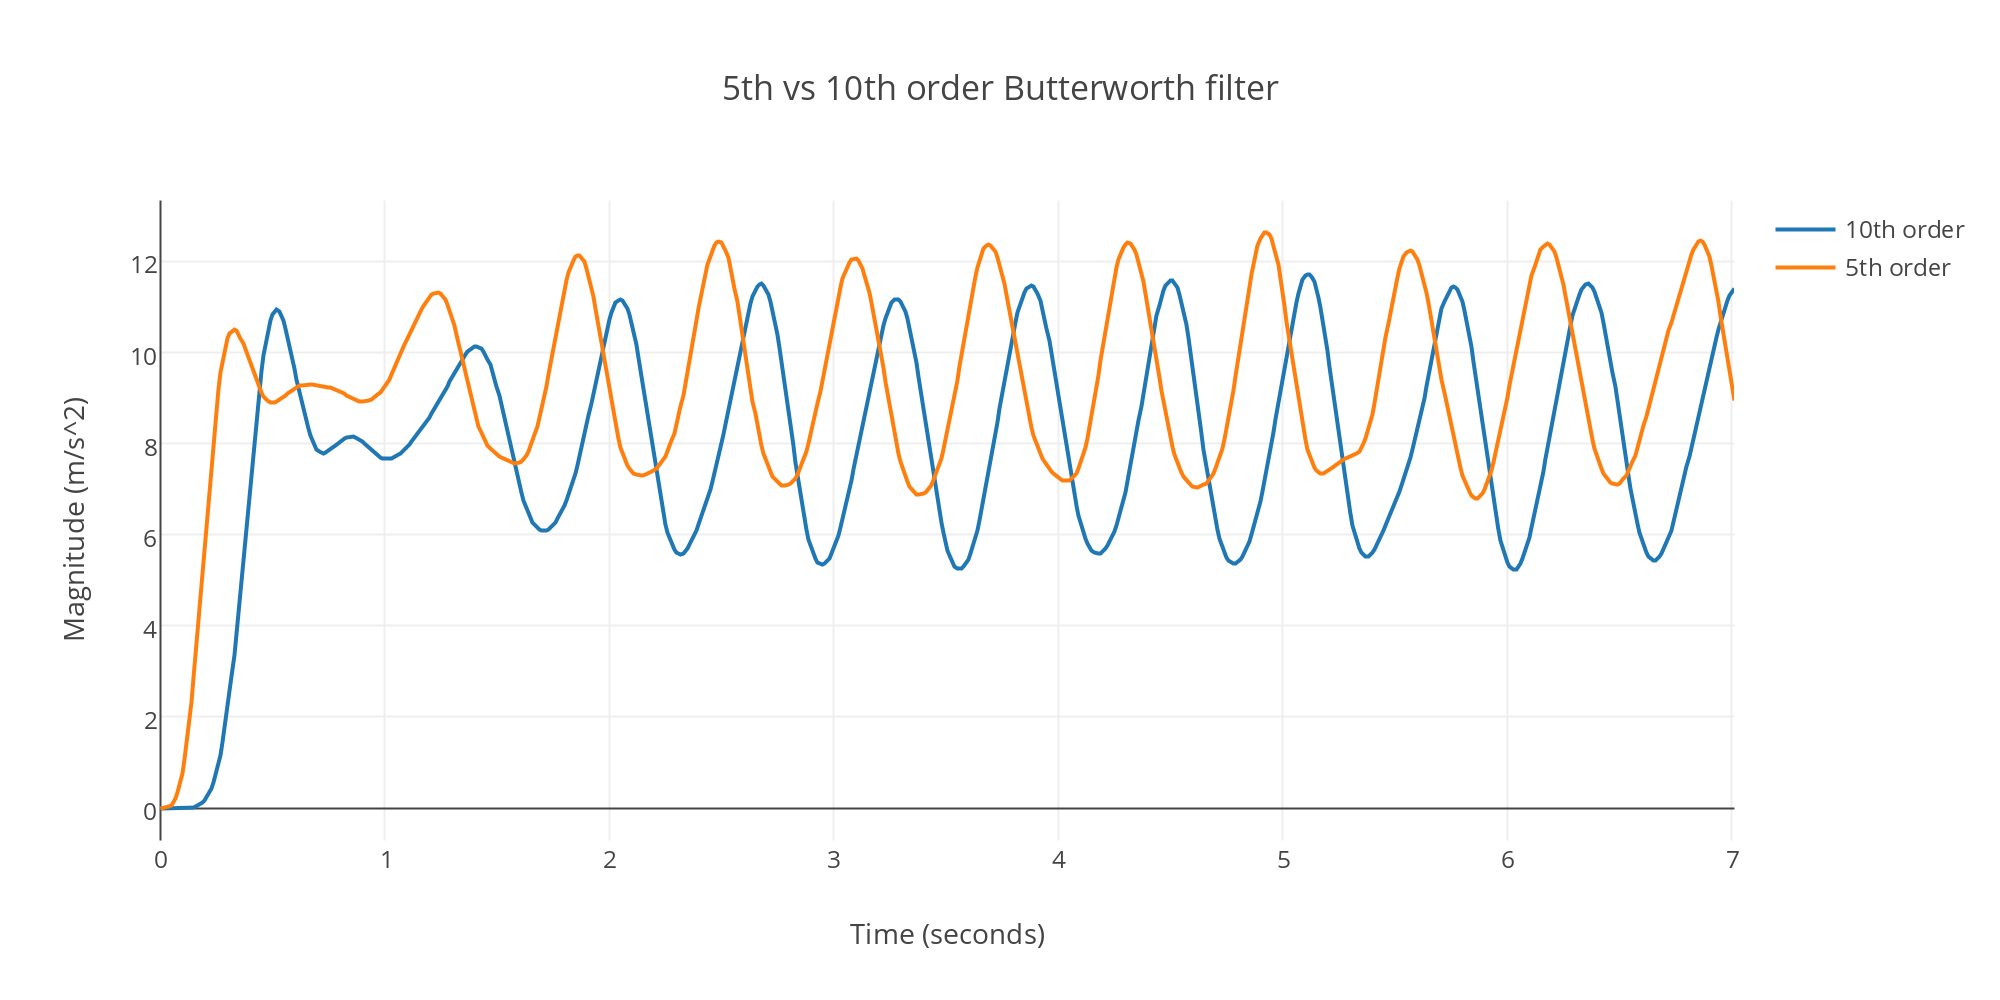
\includegraphics[scale=0.9]{images/butterworth5thVs10thOrderWalkingMagnitude.png}
\captionof{figure}{Comparing 5th and 10th order Butterworth Filters}
\label{fig:butterworth5thVs10thOrderWalkingMagnitude}
\end{center}

The shape of the 5th-order filter plot is almost identical to that of the 10th-order one, and all its peaks occur beforehand in tandem with when the steps are actually taken. Thus this 5th-order low-pass Butterworth filter is selected as the final one to use. 

\section*{Vertical acceleration}

The magnitude of the 3-axis accelerometer readings was chosen as the measure for the step detection algorithm as it is a scalar quantity and thus independent of direction. This allowed step detection to be performed in the same manner regardless of the orientation of the phone. However, it is this directional independence that also poses a problem. The vertical acceleration of the user caused during their up and down movement while walking is the basis on which steps are identified; the horizontal acceleration does not provide any meaningful information in this regard. A scalar quantity like magnitude however is unable to differentiate between vertical and horizontal accelerations. Thus periodic movement of the phone in any direction, including purely sideways, can cause steps to be fired and contribute to false positives. The filtered accelerometer magnitude output when periodically moving the phone sideways from left to right is shown in Figure~\ref{fig:butterworth5thOrderFilterSidewaysMotionMagnitude}. 

\begin{center}
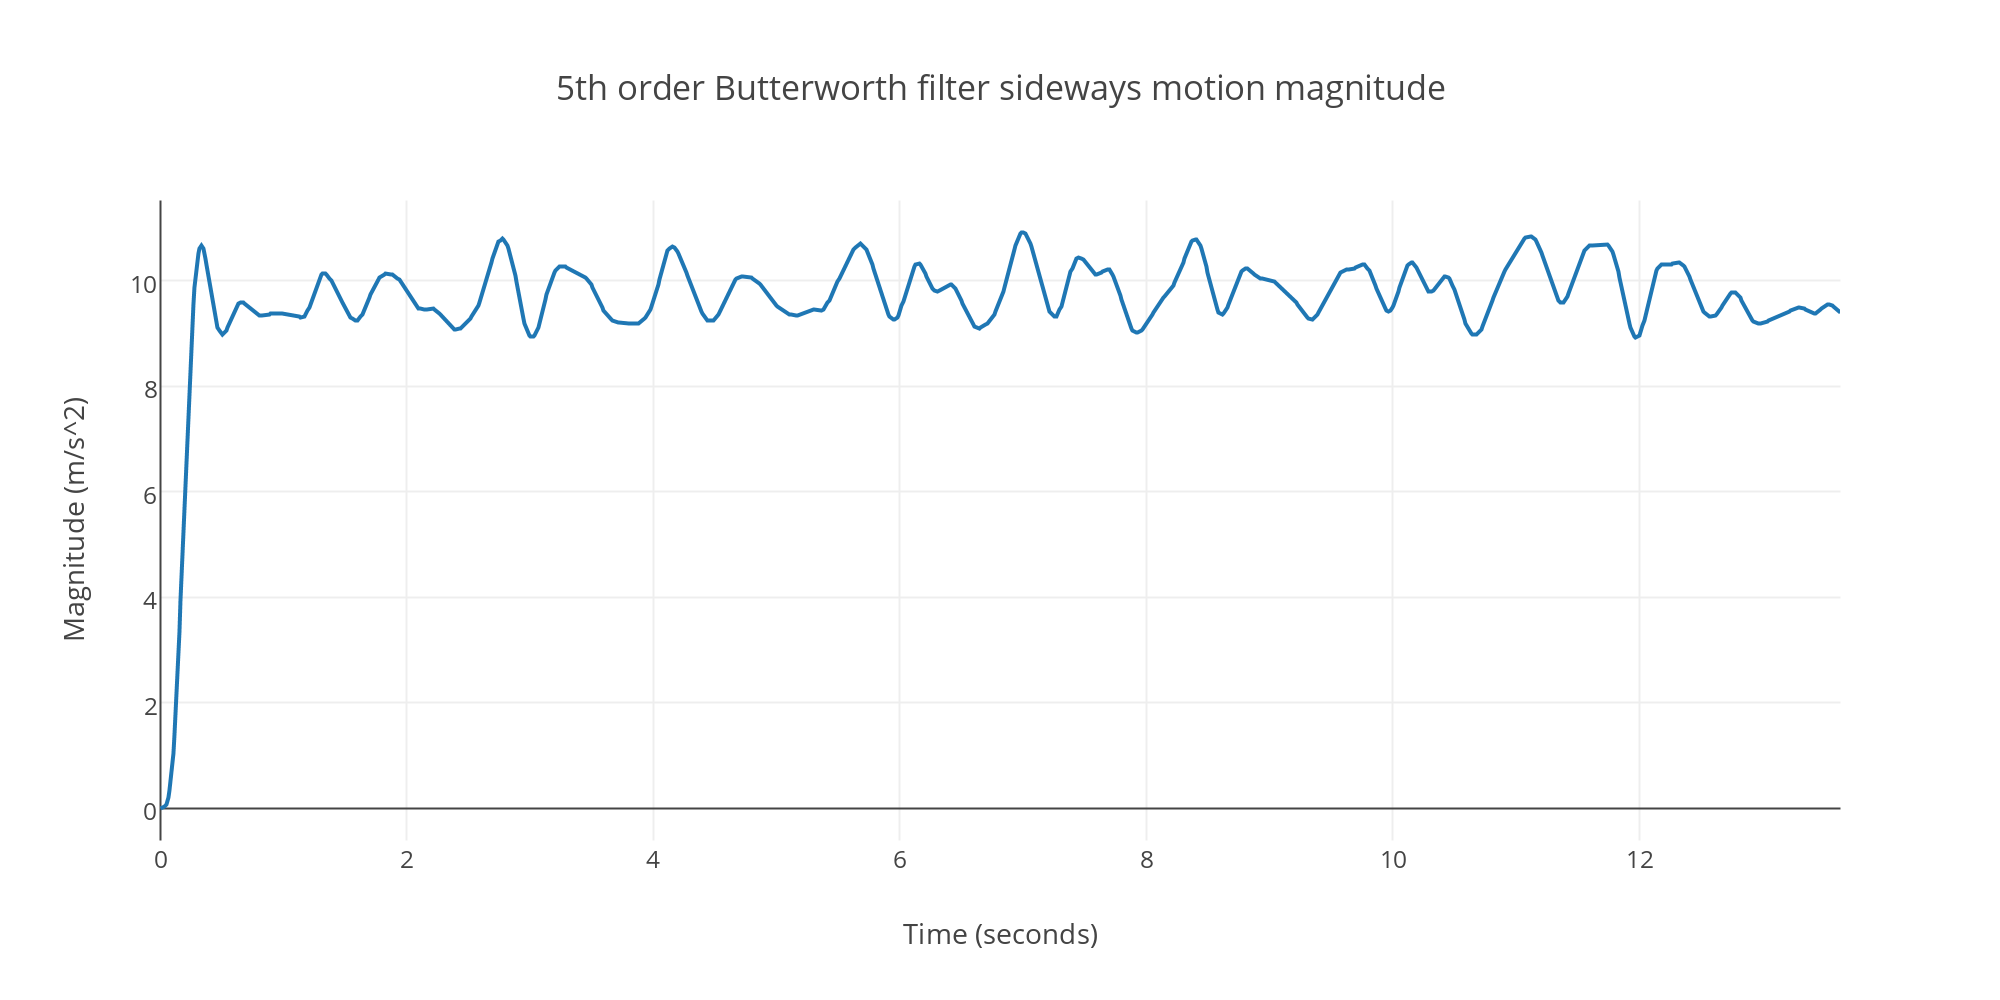
\includegraphics[scale=0.9]{images/butterworth5thOrderFilterSidewaysMotionMagnitude.png}
\captionof{figure}{Sideways motion magnitude}
\label{fig:butterworth5thOrderFilterSidewaysMotionMagnitude}
\end{center}
Thus it can be seen that it is difficult to determine on the basis of magnitude whether the variation in acceleration is due to the vertical component corresponding to walking motion or the horizontal component associated with other random motions. 

This problem is overcome by specifically tracking just the vertical component of the user's acceleration and using that as the measure for step detection. This is done by transforming the accelerometer readings from the device's local co-ordinate system to the world `East-North-Up (ENU)' co-ordinate system. The ENU system is depicted in Figure~\ref{fig:ENU}. 

\begin{center}
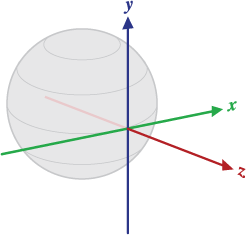
\includegraphics[scale=0.5]{images/ENU.png}
\captionof{figure}{The 3 axes in the ENU world co-ordinate system defined with respect to the Earth~\cite{ENU}}
\label{fig:ENU}
\end{center}
The Z-axis in the ENU system is defined to be pointing towards the sky and perpendicular to the surface, along the direction of the Earth's gravity vector. The Y-axis points towards the magnetic North Pole while the X-axis is defined to be the cross product of Y and Z, meaning that it roughly points East and is perpendicular to both the other axes~\cite{ENU}. From this definition it is evident that the vertical component of the user's acceleration in this system will be along the Z-axis, and thus exclusively using these readings would allow for any horizontal acceleration to be excluded from step detection. 

The mapping from the device to world ENU co-ordinates is achieved through use of a rotation matrix. This rotation matrix is obtained from a combination of the phone's gravity and magnetometer sensor readings, which provide the necessary orientation information to compute the matrix. The accelerometer readings in device co-ordinates are then multiplied by the inverse of this rotation matrix to convert them to the ENU system. Figure~\ref{fig:straightWalkVerticalAcceleration} provides an example of the filtered accelerometer readings for normal walking motion after mapping them to the ENU system. 

\begin{center}
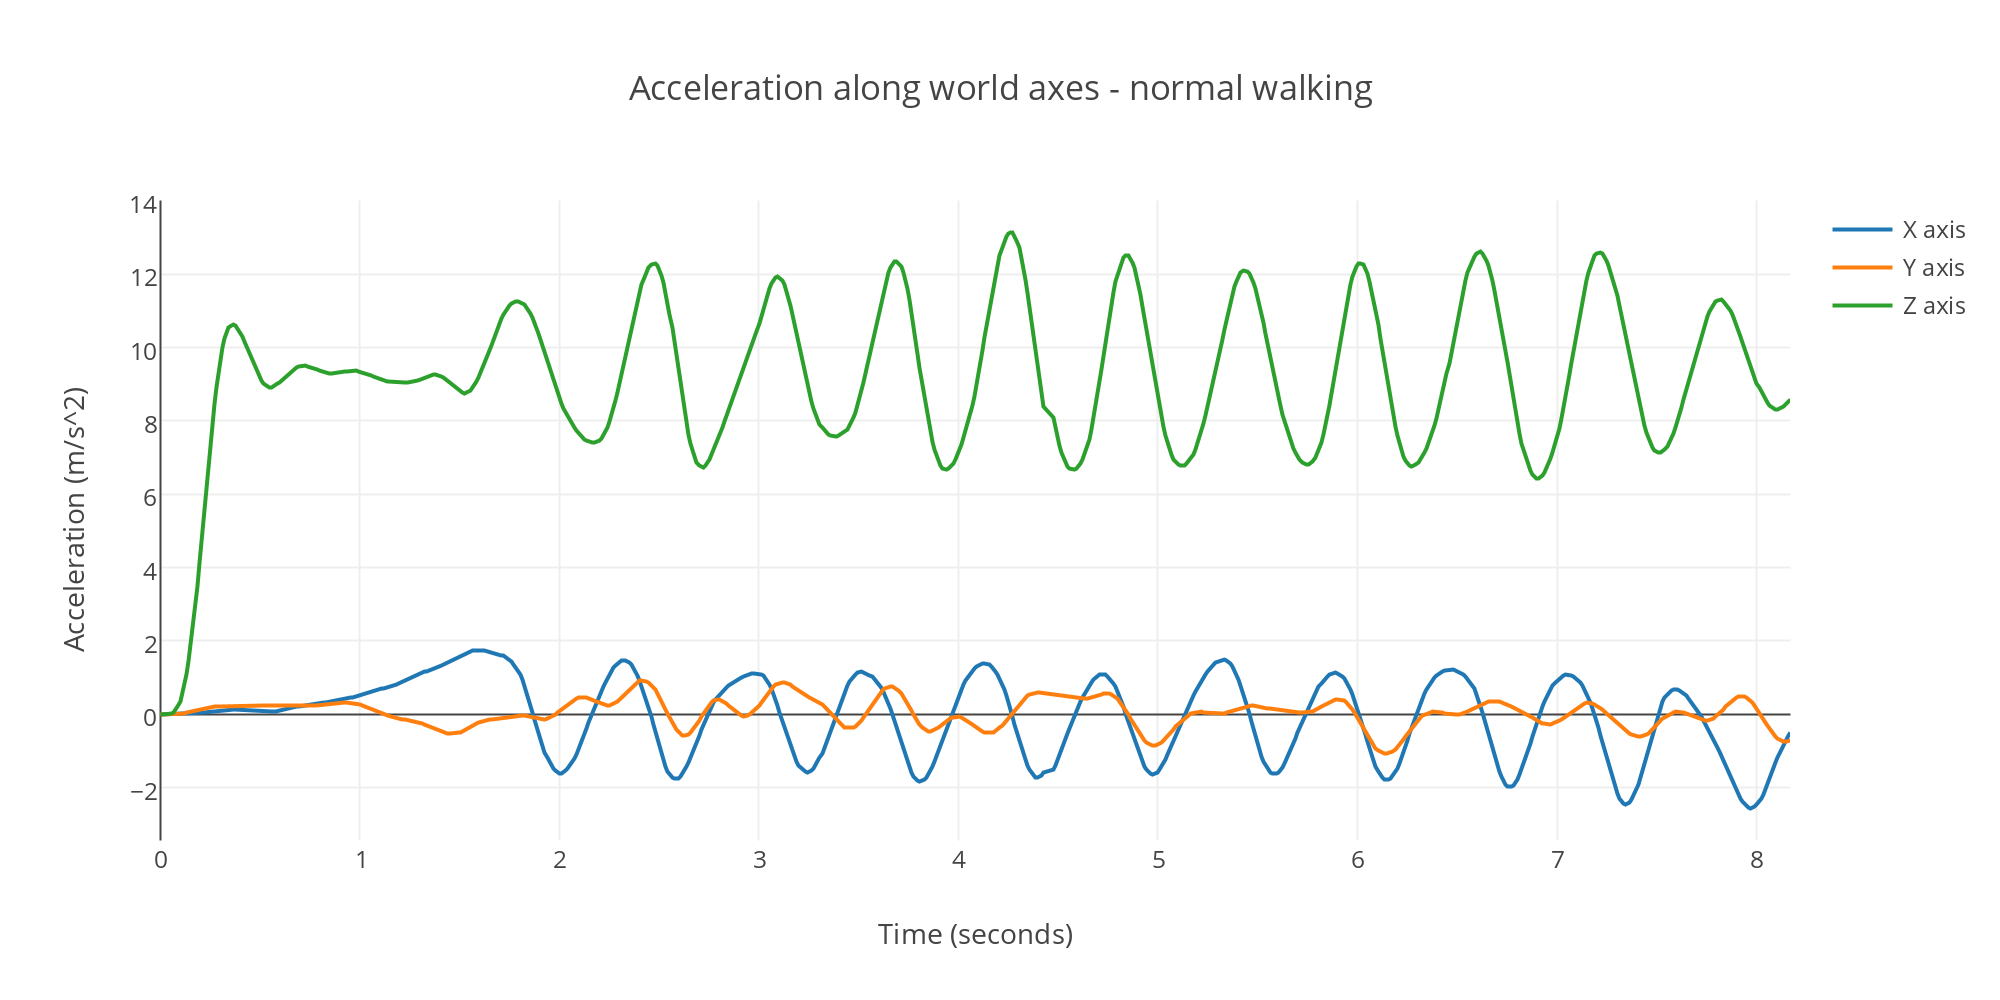
\includegraphics[scale=0.9]{images/straightWalkVerticalAcceleration.png}
\captionof{figure}{Accelerometer readings in ENU system for normal walking}
\label{fig:straightWalkVerticalAcceleration}
\end{center}
As seen in the plot, the Z-axis readings represent the user's vertical acceleration and thus fully defines the walking motion through peak/valley formation for the purpose of step detection. The Y-axis readings largely remain around 0 as the forward acceleration during walking is negligible, while the X-axis readings exhibit some variation due to the slight sidewards sway of the body while taking steps. Thus step detection can be carried out solely on the basis of the ENU Z-axis accelerometer readings.  

The robustness of this approach with respect to the magnitude readings is demonstrated by Figure~\ref{fig:sidewaysMotionVerticalAcceleration}, which depicts the filtered accelerometer output when moving the phone in a sideways manner.  

\begin{center}
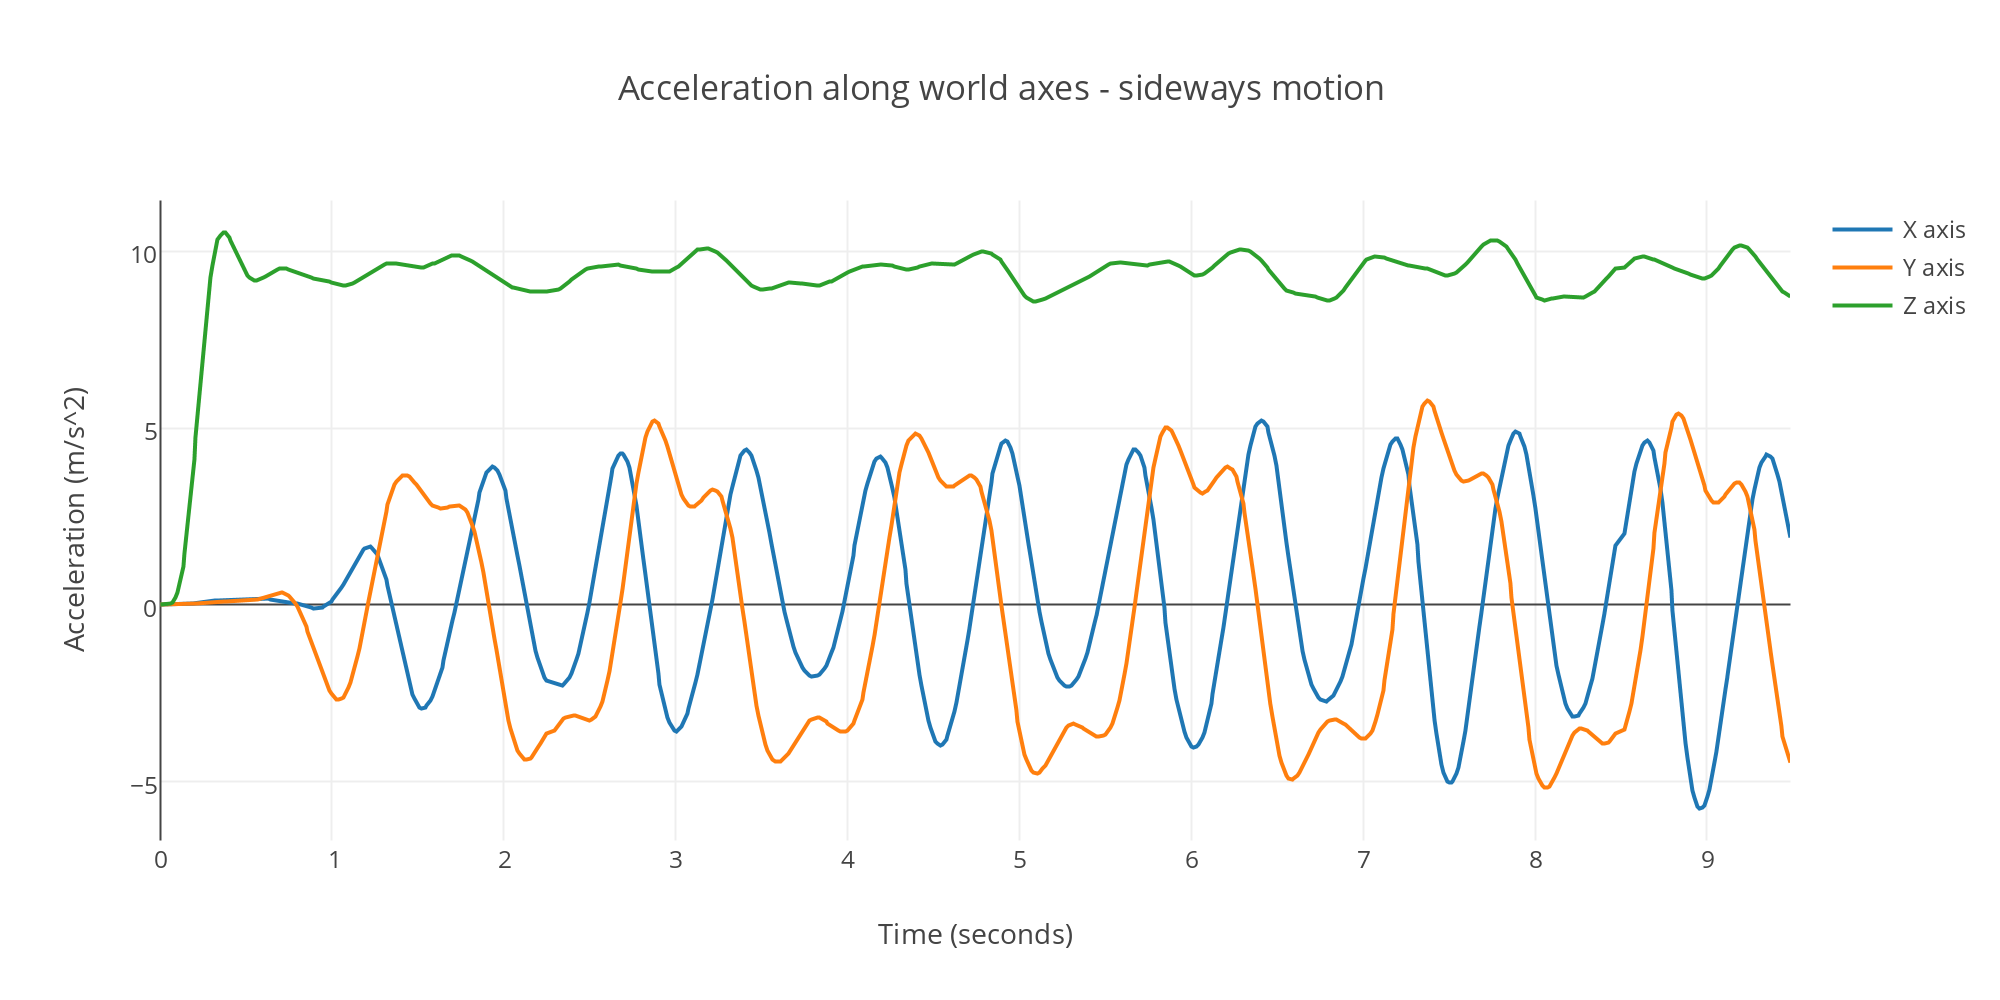
\includegraphics[scale=0.9]{images/sidewaysMotionVerticalAcceleration.png}
\captionof{figure}{Accelerometer readings in ENU system for sideways motion}
\label{fig:sidewaysMotionVerticalAcceleration}
\end{center}
In this case the variations are along the X and Y axes. The Z-axis readings however remain largely flat since sideways motion does not produce vertical acceleration. Thus it is far more unlikely for such movements to result in false positives in the ENU system as compared to using the magnitude of the acceleration for step detection. 

\section*{Further Optimisations}

Using the Butterworth filter and accelerometer readings in the ENU system results in step detection that is accurate and responsive while also being fairly robust to false positives. However there are still occasional cases where unrelated movements cause steps be recorded. Thus the following additional constraints derived from characteristics of typical human gait are applied to further reduce the likelihood of false positives occurring.  

\subsection*{Thresholding}

A minimum threshold $t_{min}$ for the absolute difference between adjacent valley/peak accelerations was discussed in the previous section for differentiating between momentary hand motions and normal walking motion. This minimum threshold also ensures that very slight fluctuations in acceleration value due to noise or any other external factors do not trigger a step. This idea can be extended by noticing the fact that the accelerations produced by standard walking usually lie within a certain fixed interval. Any acceleration considerably larger than the maximum value of this interval is likely to have been generated from a motion other than walking. Thus a maximum threshold $t_{max}$ is also applied to the accelerometer readings. The difference between an adjacent valley and peak must be above $t_{min}$ and below $t_{max}$ for it to be recorded as a step. 

\subsection*{Peak to valley difference}

Steps are currently detected solely on the basis of the acceleration difference from a valley to its corresponding peak. The absolute acceleration in the downward phase of a step is expected to be roughly similar to that in the upward phase for standard walking. Thus the condition that the peak to valley difference must be within a certain percentage of the preceding valley to peak difference for it to be classified as a step is introduced. This means that any step is now actually recorded at the valley following the peak.   

\subsection*{Time difference}

It was noted in the previous section that the frequency of normal walking motion ranges between 0.7-3 Hz. Assuming 3 steps to be the maximum taken per second during walking means that the time interval between subsequent steps is at least approximately 330ms. Any smaller time difference suggests that the recorded motion is too quick for it to be standard walking. Thus allowing for a small margin, a minimum requirement of 300ms between consecutive steps is set in the application. If a valley is found to occur before 300ms have passed since the previous one, the step associated with it is ignored and not added to the overall count.

\nocite{*}

\bibliography{StepDetection}
\bibliographystyle{plain}

\end{document}